\chapter{基于跨模态文本重构的神经机器翻译}
% 本文应该侧重的是:
%    明确的视觉信息融合方式;
%    短语和词级别的视觉信息融合;
%    模型不需要对视觉信息敏感,因为视觉信息直接作用到目标上了

% 摘要
% 原文摘要:现有多模态机器翻译将视觉信息以全局特征的方式作为固定上下文输入,或者利用注意力机制对图像建立动态上下文作为文本内容的补充信息。然而这种隐含式的视觉信息融合方法对于分析图像如何起到作用以及为什么会产生作用带来了很大的挑战。针对此问题,提出了一种实体级的跨模态信息融合方法,显式地将文本中实体替换为对应图像中的视觉目标,并利用翻译模型来重建出完整的原文本,最后通过多任务的方式将以上重建任务与翻译任务相结合。实验表明,该方法在有效的提升了实体词的翻译质量,译文质量得到了显著的提升。
% 
%现有融入图片信息的神经机器翻译将视觉信息以全局特征的方式作为固定上下文输入,或者利用注意力机制对图像建立动态上下文作为文本内容的补充信息。然而这种隐含式的视觉信息融合方法对于分析图像如何起到作用以及为什么会产生作用带来了很大的挑战。针对此问题,提出了一种实体级的跨模态信息融合方法,显式地将文本中实体替换为对应图像中的视觉目标,并利用翻译模型来重建出完整的原文本,最后通过多任务的方式将以上重建任务与翻译任务相结合。实验表明,该方法在有效的提升了实体词的翻译质量,译文质量得到了显著的提升。

% 神经机器翻译中融合图片信息的问题:普遍范式中,句子与图片的信息融合是隐式的,即无法准确得知视觉信息作用到哪些词上或对句子的表示带来了哪些影响,因此,为了探索是否能够以明确的方式融合视觉信息,明确方式融入视觉信息是否对翻译有效,本章提出了一种在名词短语或名词的粒度上融合图片中的视觉目标信息,并进行跨模态文本重构的重构任务。再通过多任务训练的方式,将重构任务所优化的模型参数与翻译任务共享,从而达到提升翻译质量的目的。本章设置了进一步的分析实验,实验结果表明本章所提方法通过有效的提升实体词的翻译质量,从而提升了翻译准确率。

% 多模态的好处
采用分布式向量表示的神经翻译模型和计算机视觉基础模型极大地便利了以句子为基本语义单位的跨模态信息融合,
% 研究现状
例如,将图片以全局特征的方式作为固定上下文输入到神经翻译模型中,或者利用注意力机制对图像建立动态上下文作为文本内容的补充信息。
% 存在的问题
然而在这些方法中,句子与图片的信息融合是隐式的,即无法准确得知视觉信息作用到哪些词上或对句子的表示带来了哪些影响。
% 本章提出的方法
因此,为了探索是否能够以明确的方式融合视觉信息,以及明确方式融入视觉信息是否能够带来稳定的翻译质量提升,本章提出了在词级和短语级融合图片中的视觉目标信息,并进行跨模态文本重构的重构任务。通过多任务训练的方式,将文本重构任务所优化的模型参数与翻译任务共享,从而达到提升翻译质量的目的。
% 进一步的分析结果
%本章设置了进一步的分析实验,实验结果表明本章所提方法通过有效地提升实体词的翻译质量,从而提升了翻译准确率。
本章设置了进一步的分析实验,实验结果表明所提方法对实体词的翻译有更好的提升效果,从而提升了译文的质量。

\section{引言}
% 背景:
得益于神经网络方法的快速发展,自然语言处理和计算机视觉等领域均得到了飞速的进步,同时也为跨模态的信息融合带来了可能。在神经机器翻译中融合图片信息就是跨模态信息融合方法的一类应用。这类方法是为了解决一些在翻译中难以处理的问题,例如文本中存在歧义,句子表达不完整,低频词的欠拟合等问题。图片中往往包含着更丰富的语义信息。因此,如何将图片信息融合到翻译中成为了研究者们所关注的问题,相关方法也层出不穷。

% 相关研究:
目前已有的研究主要关注如何将整个图片中的信息融合到神经机器翻译模型的翻译过程中。由于图像分类任务所使用的卷积神经网络,如Resnet-50\cite{32_DBLP:conf/cvpr/HeZRS16},取得了非常好的效果,因此多数研究这尝试将预训练的卷积神经网络与神经翻译模型相结合。例如部分研究将图片经过卷积神经网络提取得到全局特征后,将其作为一个包含完整的上下文信息的特征向量以各种方式输入到翻译模型中,从而完善翻译模型在编码过程所获得的语义表征或为解码过程提供外源信息以供参考\cite{52_DBLP:journals/corr/ElliottFH15,18_DBLP:conf/emnlp/CalixtoL17,22_li-etal-2021-vision,20_wu-etal-2021-good}。
文献\cite{36_calixto-etal-2017-doubly,47_DBLP:conf/wmt/LibovickyHM18}尝试利用图片局部特征与注意力机制配合获图片的局部动态上下文,以达到在解码过程中融合与当前解码步骤最相关的视觉信息。此类方法中,图片作为一个句子级别的语义信息提供者作用到翻译过程中,试图使翻译模型最大化地利用图片中所包含的信息。
%因视觉信息与文本信息的融合与利用为通过模型学习的方式,而难以明确图片信息在翻译中的作用过程,本文称此类方法为隐式跨模态信息融合方法。

% 存在的问题:
然而,这些方法均以隐式的方式将图片信息与文本信息相结合,这些融合图片信息的神经机器翻译模型是如何应用视觉信息,以及为何输入图片能够使得翻译性能提升都是不明确的,本文中,我们称此类方法为隐式跨模态信息融合方法。
值得注意的是,将图片输入到翻译模型中并不能保证模型翻译质量的提升,部分融合图片信息的翻译模型相比于对应的纯文本基线模型提升的翻译性能几乎是可以忽略的\cite{53_caglayan-etal-2019-probing}。
%更重要的是,部分方法存在翻译质量提升不稳定的情况,不同的模型实现方案或不同的模型初始化条件下模型的翻译性能表现差异较大。
尽管在句子级语义单位可以最大化地利用图片中所携带的视觉信息,但神经翻译模型似乎不能很顺利地将其利用。

% 本章提出方法
为此,本章提出了一种基于跨模态文本重构的神经机器翻译方法(neural machine translation based on cross-modal text reconstruction, CTR-NMT),以显式方式融合跨模态信息。文献\cite{53_caglayan-etal-2019-probing}发现,当文本中部分内容或信息缺失,尤其是实体词缺失时,神经翻译模型对视觉信息最敏感。为了将图片中的视觉信息明确并有效地融合到模型中,本章以实体为语义单元融合图片信息,其中实体在句子中以词级或短语级两种方式呈现。区别于文献\cite{53_caglayan-etal-2019-probing}通过创造的文本内容缺失环境提升隐式跨模态信息融合有效性,本文采用显式跨模态信息融合方法,直接利用视觉特征替换实体后用作模型输入,规避了视觉信息在神经机器翻译模型中难以有效作用的问题。为了实现跨模态的信息融合,本章设计了一个文本重构模型来实现跨模态输入到纯文本输出的生成任务。该模型将实体被视觉目标替换掉的源语言句子作为输入,以完整的源语言句子或参考译文作为输出,通过端到端的学习将视觉目标中的视觉信息融合到实体的表示中。最后,本文将跨模态的文本重构任务与翻译任务相结合,通过多种参数共享机制,使翻译模型能够充分利用到从文本重构任务中学习到的视觉信息,从而提升模型的翻译质量。

本章主要贡献如下:

(1)本章提出了一种基于跨模态文本重构的神经机器翻译方法, 并且将所提方法应用到了基于循环神经网络和基于Transformer的两种神经机器翻译框架中。本章详细对比了多种参数共享方案,在测试阶段没有额外的图片输入的情况下,达到了与其它模型可比的翻译准确率。并且与纯文本基线模型相比,有着显著的翻译质量提升。

(2)本章提出了一种显式跨模态信息融合法,即以明确的方式将图片信息融合到文本的表示与生成中。该方法将图片中的视觉目标信息明确作用到句子中相对应的实体上,并在词级和短语级两种粒度的跨模态融合方案进行了实验对比,发现相比于短语实体,在词实体上融合图片信息效果更佳。

(3)本章对视觉目标的作用对象进行了分析,并发现本章所采用的明确的图片信息作用方法,使名词实体的翻译准确率获得了更多的提升,进而提升了神经机器翻译模型的翻译质量。

\section{相关工作}

% 相关工作分类:
%     传统方法:句子级融合法,隐式法,(Feature-level Incongruence Reduction for Multimodal Translation,直接使用视觉特征不适合当前模型)
%     重构法:文本重构(Neural Machine Translation with Reconstruction,
%            图像重构(mywork2)(Imagination,Adversarial reconstruction for Multi-modal Machine Translation
%     实体替换法:主要用于分析
%     视觉目标法:
%     预训练模型法:包含纯文本预训练模型,毕竟消融实验中有类似的

% 这里可能需要提一下“退化文本”的概念

% 

本章工作主要目标是将图片中的视觉目标信息通过文本重构方法融合到文本的表示中,相关工作主要包含以下两个部分:

{\sffamily (1)融合视觉目标信息的神经机器翻译}

本文在\ref{sec:2_cv}小节中提到,在文本中融合图片信息的方式有很多中,其中采用图片中视觉目标信息的方式过滤掉了大部分无用的背景信息。
\tcite{huang2016attention}尝试了将图片中的多个视觉目标提取出来形成一个序列,拼接到源语言句子的词向量序列后面,再输入到模型中进行端到端的翻译。该工作还尝试将每个视觉目标与源语言句子单独进行编码的方案,然后采用注意力机制去关注与当前解码词最相关的那个编码序列,从而动态地利用视觉目标信息。
\tcite{yin2020novel}将句子与图片中的视觉目标视为图的关系,采用基于图的编码器融合跨模态信息。
\tcite{wang2021efficient}将视觉目标传递给翻译模型后,为了使模型利用到与文本内容相关的视觉信息并排除内容不相关的视觉信息,设计了目标掩码损失函数(object-masking loss)和视觉权重翻译损失函数(vision-weighted translation loss),分别在编码阶段和解码阶段针对文本的内容将视觉目标进行掩码或打分。

虽然采用视觉目标信息的方法能够避免引入大量的噪音信息,但是在文本信息和视觉信息融合的过程中,模型仍然需要学习如何主动地将图片中的有效信息整合到翻译的编码或解码过程中。然而,图片信息在这个过程中的具体作用并不清楚,信息融合的方式也是隐式的。与这些方法不同,本章采用了显式跨模态信息融合方法,直接将视觉目标信息应用到与之相关的单词或短语上。

{\sffamily (2)基于图片信息的文本生成}

融合图片信息的神经机器翻译任务与基于图片信息的文本生成任务素有渊源。基于图片信息的文本生成常指图片描述生成(image captioning)任务,即给定一张图片生成与图片内容相关的句子。\tcite{vinyals2015show}使用了一个基于长短时记忆网络(long short-term memory, LSTM)的编码器-解码器模型来生成图片描述,它首先用一个卷积神经网络将图片编码成一个固定长度的向量,然后用一个LSTM将向量解码成一个自然语言句子。\tcite{xu2015show,lu2017knowing}进一步地在编码器-解码器模型中加入了注意力机制,使模型在解码的过程中能够动态地关注图片中的局部信息,从而生成更丰富的描述。从这些方法的特点不难看出,融合图片信息的神经机器翻译方法从中得到了很多的启发。\tcite{kiros2014unifying}将图片描述生成定义为图片翻译任务,并在描述生成的过程中加入了源语言句子。\tcite{calixto2017doubly}在文本注意力的基础上增加的图片注意力与图片描述生成所采用的方法相似。

%文献\cite{53_caglayan-etal-2019-probing}采用掩码的方式将源语言句子中的颜色、实体词和文本序列片段替换为没有明确含义的掩码词“<mask>”,从而得到退化文本(degrade text),然后在输入正确以及错误图片信息的情况下观察翻译模型的性能变化,发现当文本中缺失信息,尤其是实体词信息缺失时图片信息在模型中起了明显的作用。本章采用的基于图片信息的文本生成方法就是将视觉目标与退化文本相结合,并用结合后的多模态序列生成源语言或目标语言的文本。
\tcite{caglayan2019probing}通过使用掩码词“<mask>”替换源语言句子中的颜色、实体词和文本片段等关键信息,构造了退化文本(degraded text),然后分别在给定正确和错误的图片信息的条件下评估翻译模型的性能变化。结果表明,当文本中信息丢失时,特别是实体词信息时,图片信息对模型对模型性能的影响较大。本章采用了一种基于图片信息的文本生成方法,它将视觉目标与退化文本结合起来,并利用多模态序列生成源语言或目标语言的完整文本。


%目前,融合图片信息的神经机器翻译方法多采用将图片输入到翻译模型中辅助翻译过程的方式,但得到的翻译性能提升并不理想。相比之下,利用图片信息优化翻译模型参数进而增强翻译性能的方法取得了稳定且有效的提升。文献【】
\section{实体对齐方法}
\label{sec:3_entity_extraction}
% 我们需要的是什么样的视觉特征,以及为什么
本章所提方法是针对名词短语或名词融合图片中的视觉信息。也有相关工作尝试以词为粒度融合视觉信息,例如\tcite{wu2021good,li2021vision}均采用了门控机制来控制图片的全局特征与输入序列中每个单词的隐层表示的融合。然而,这种方式为模型所提供的图片信息依旧是不明确的。为此,我们选择将图片中与名词或短语相对应的视觉目标提取出来再进行信息的融合。该过程涉及到如何将句子中的名词或短语与图片中的视觉目标对齐。图\ref{fig:3_entity_extraction}为本文的解决方案。
\begin{figure}[!htbp]
    \centering
    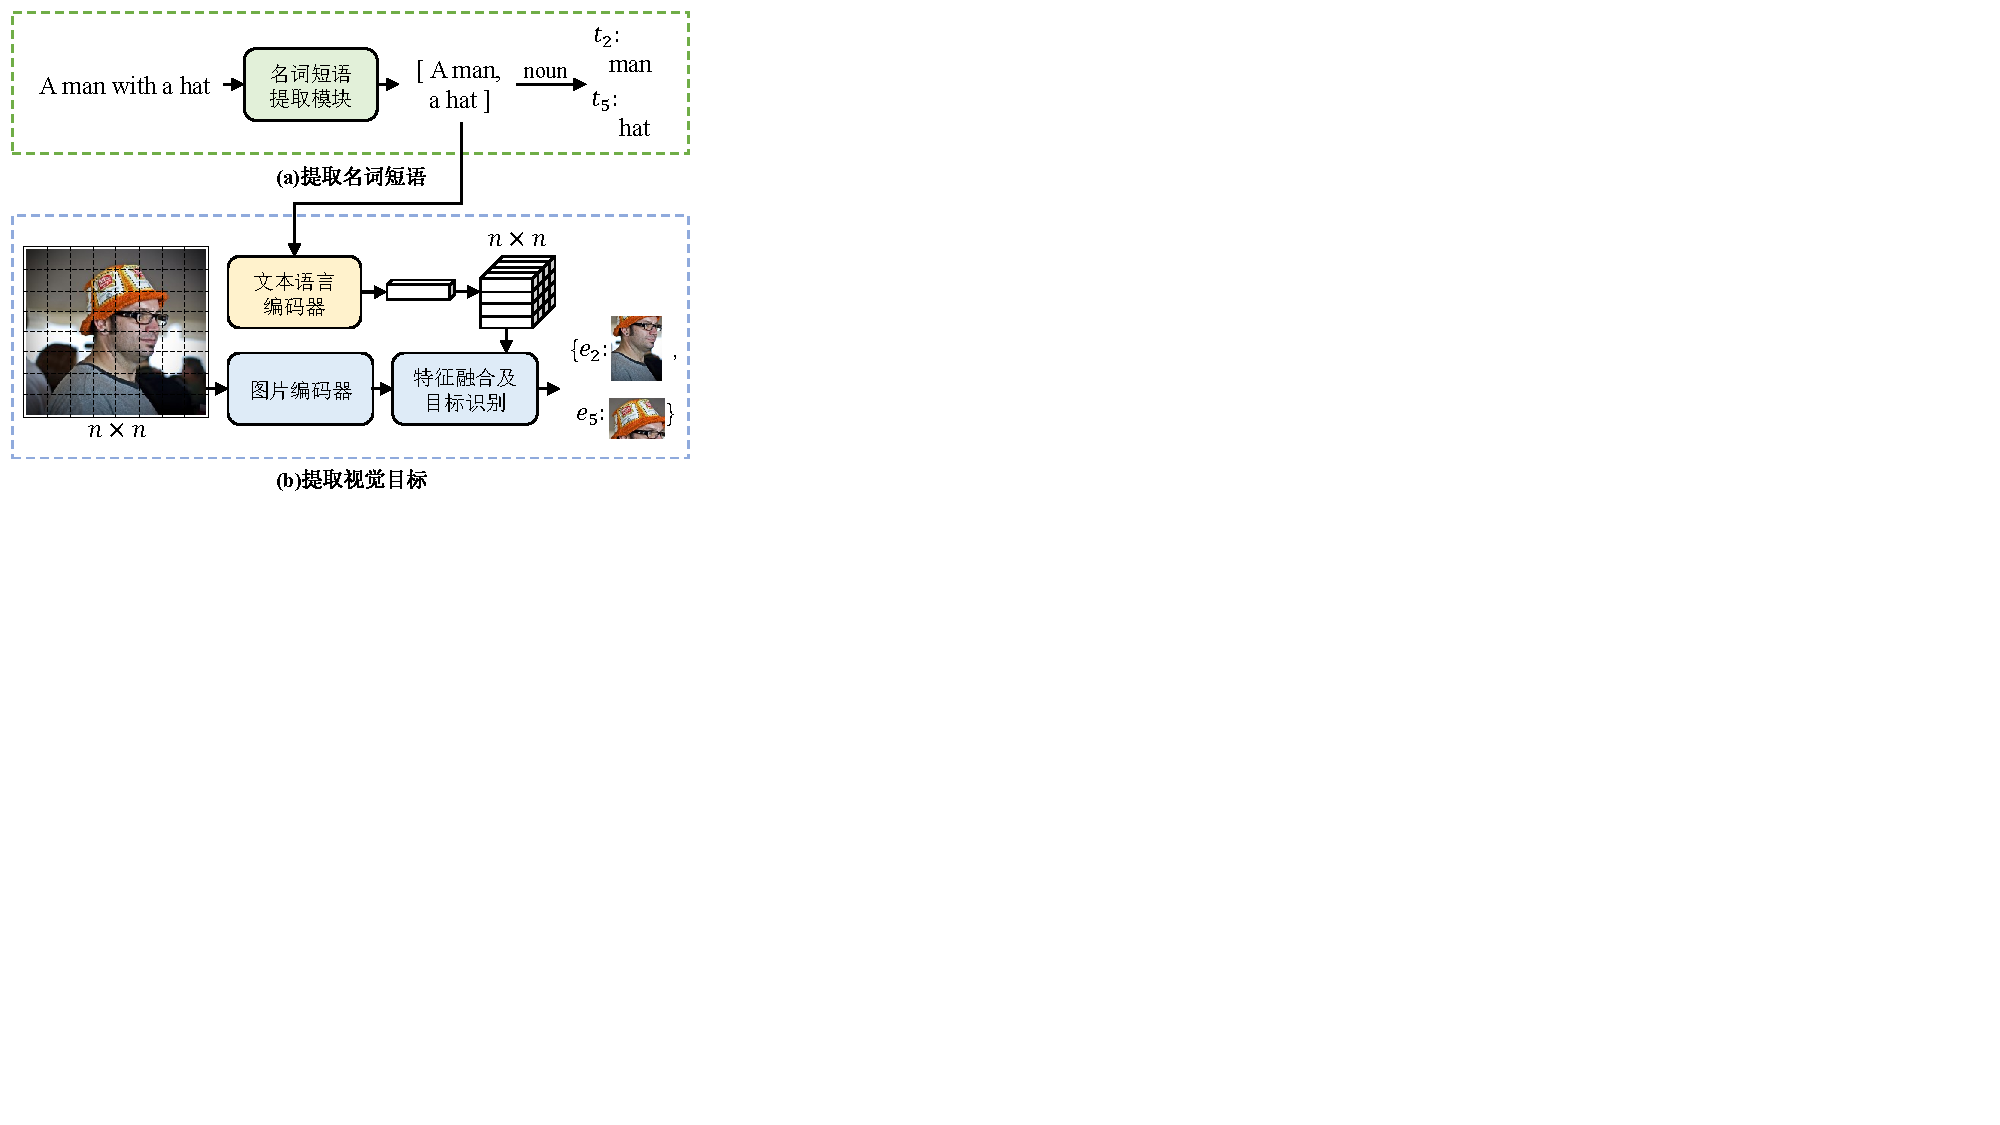
\includegraphics{Img/fig_3_entity_extraction.pdf}
    \bicaption{实体提取与对齐方法}{Entity extraction and alignment methods}
    \label{fig:3_entity_extraction}
\end{figure}

图\ref{fig:3_entity_extraction}a展示了名词短语的提取过程。本文采用成熟的spaCy\footnote{https://spacy.io/}工具提取源语言句子中的名词短语。这样再通过对句子的词性标注即可获得所提取的短语中的名词。例如,将句子“A man with a hat.”输入到短语提取工具中,可得到名词短语“A man”和“a hat”,其中“man”和“hat”就是本文需要的名词。因为考虑到句子中仅名词或名词短语在图片中有着直接对应的视觉目标,所以在该方法中不考虑源语言句子中其它类型的短语。

图\ref{fig:3_entity_extraction}b展示了图片中视觉特征的提取过程。在得到了文本中的名词短语后,就可以根据这些短语提取图片中对应的区域作为视觉目标。为此,本文采用了\tcite{yang2019a}提出的单步视觉目标提取法(one-stage visual grounding)。该方法的输入是一张图片和一个短语,模型的输出为短语所对应的图片区域。简化工作流程为,利用预训练的语言模型(如BERT\pcite{devlin2019bert})和预训练的图片编码器(如Darknet-53\pcite{redmon2018yolov3})分别为短语和图片提取语义特征向量和图片栅格特征,然后将语义特征向量与栅格特征中每个栅格的特征相融合(如拼接)。将融合的特征送入检测模块判断栅格中哪些位置是属于输入的短语,最后拼接成一块完整的区域。例如,将“A man”和完整的图片输入到模型中,提取出来的就是图片中“男人”所对应的区域。

经过以上过程,就可得到源语言句子中的名词、名词短语、视觉目标以及它们之间的对应关系。
\section{方法描述}

本节将首先介绍句子和图片的输入方式,解释如何做到明确的视觉信息作用方法。然后介绍本章设计的文本重构模型是如何工作的。最后介绍如何利用文本重构模型帮助优化翻译模型参数。

\subsection{实体替换的多模态序列}
\label{sec:3_entity_replacement}

\begin{figure}[!htbp]
    \centering
    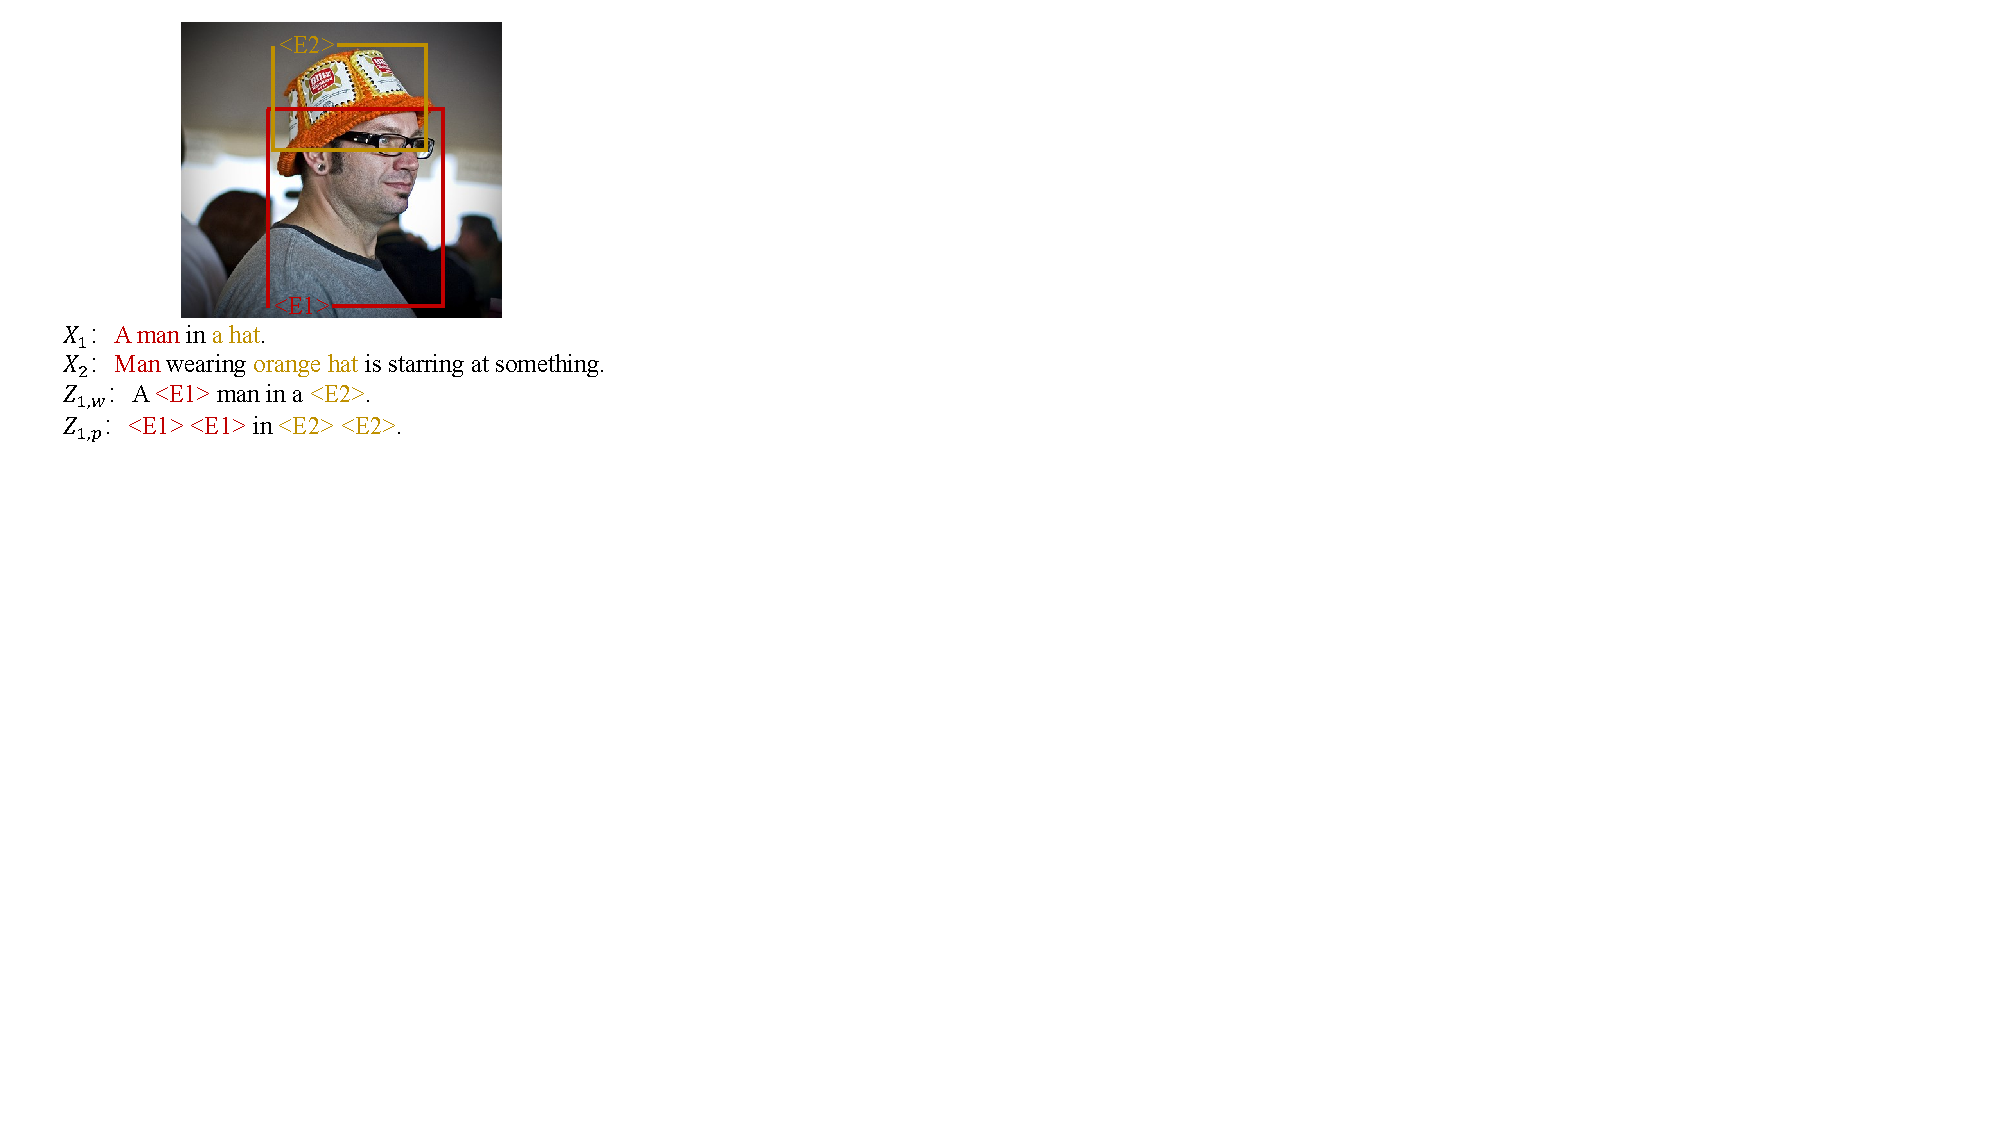
\includegraphics{Img/fig_3_example.pdf}
    \bicaption{词实体与短语实体替换示例}{An example of the word entity and the phrase entity}
    \label{fig:3_example}
\end{figure}
本章所提的显式融合方法将作用于句子中的实体,为此本文以两种语义粒度定义文本实体:

(1){\sffamily 短语实体:}一个短语实体是一个视觉可描述短语,其能够完整的描述一个视觉目标图片。例如,图\ref{fig:3_example}中红框中的人“<E1>”在句子$X_1$中被描述为“A man”。其中,“man”是视觉目标,“A”为“man”的数量修饰词,两个词对于所描述的视觉目标均是有明确意义的。

(2){\sffamily 词实体:}一个词实体是短语实体中的名词实体。对于不同的描述者,视觉目标图像可以被描述为不同的短语。如图\ref{fig:3_example}中,同样是视觉目标“<E1>”,在句子$X_2$中则被描述为“Man”,对视觉目标“<E2>”,$X_1$中描述为“a hat”,在$X_2$中则使用了修饰词描述为“orange hat”。为了消除修饰词带来的影响,在此方案中只考虑名词作为文本实体。

本章所提的显式图片信息融合方法,就是将源语言句子中的文本实体直接替换为图片中与文本实体相对应的视觉目标。
由于存在两种文本实体,因此本文设置了两种替换规则:短语级替换规则(phrase-level replacement rule,PRR)和词级替换规则(word-level replacement rule,WRR)。在PRR中,短语内部的所有词将逐个被该短语所对应的视觉目标图像替换。例如图\ref{fig:3_example}中,$Z_{1,p}$中的“A”和“man”均被替换为“<E1>”对应的视觉目标。WRR与上述方法相似。如图\ref{fig:3_example}中$Z_{1,w}$仅名词部分(“man”,“hat”)被替换为对应的视觉目标(“<E1>”,“<E2>”)。最后的输入为该退化的句子与视觉目标图像的混合序列。

\subsection{文本重构模型}
\label{sec:3_sentence_reconstruction}
\begin{figure}[!htbp]
    \centering
    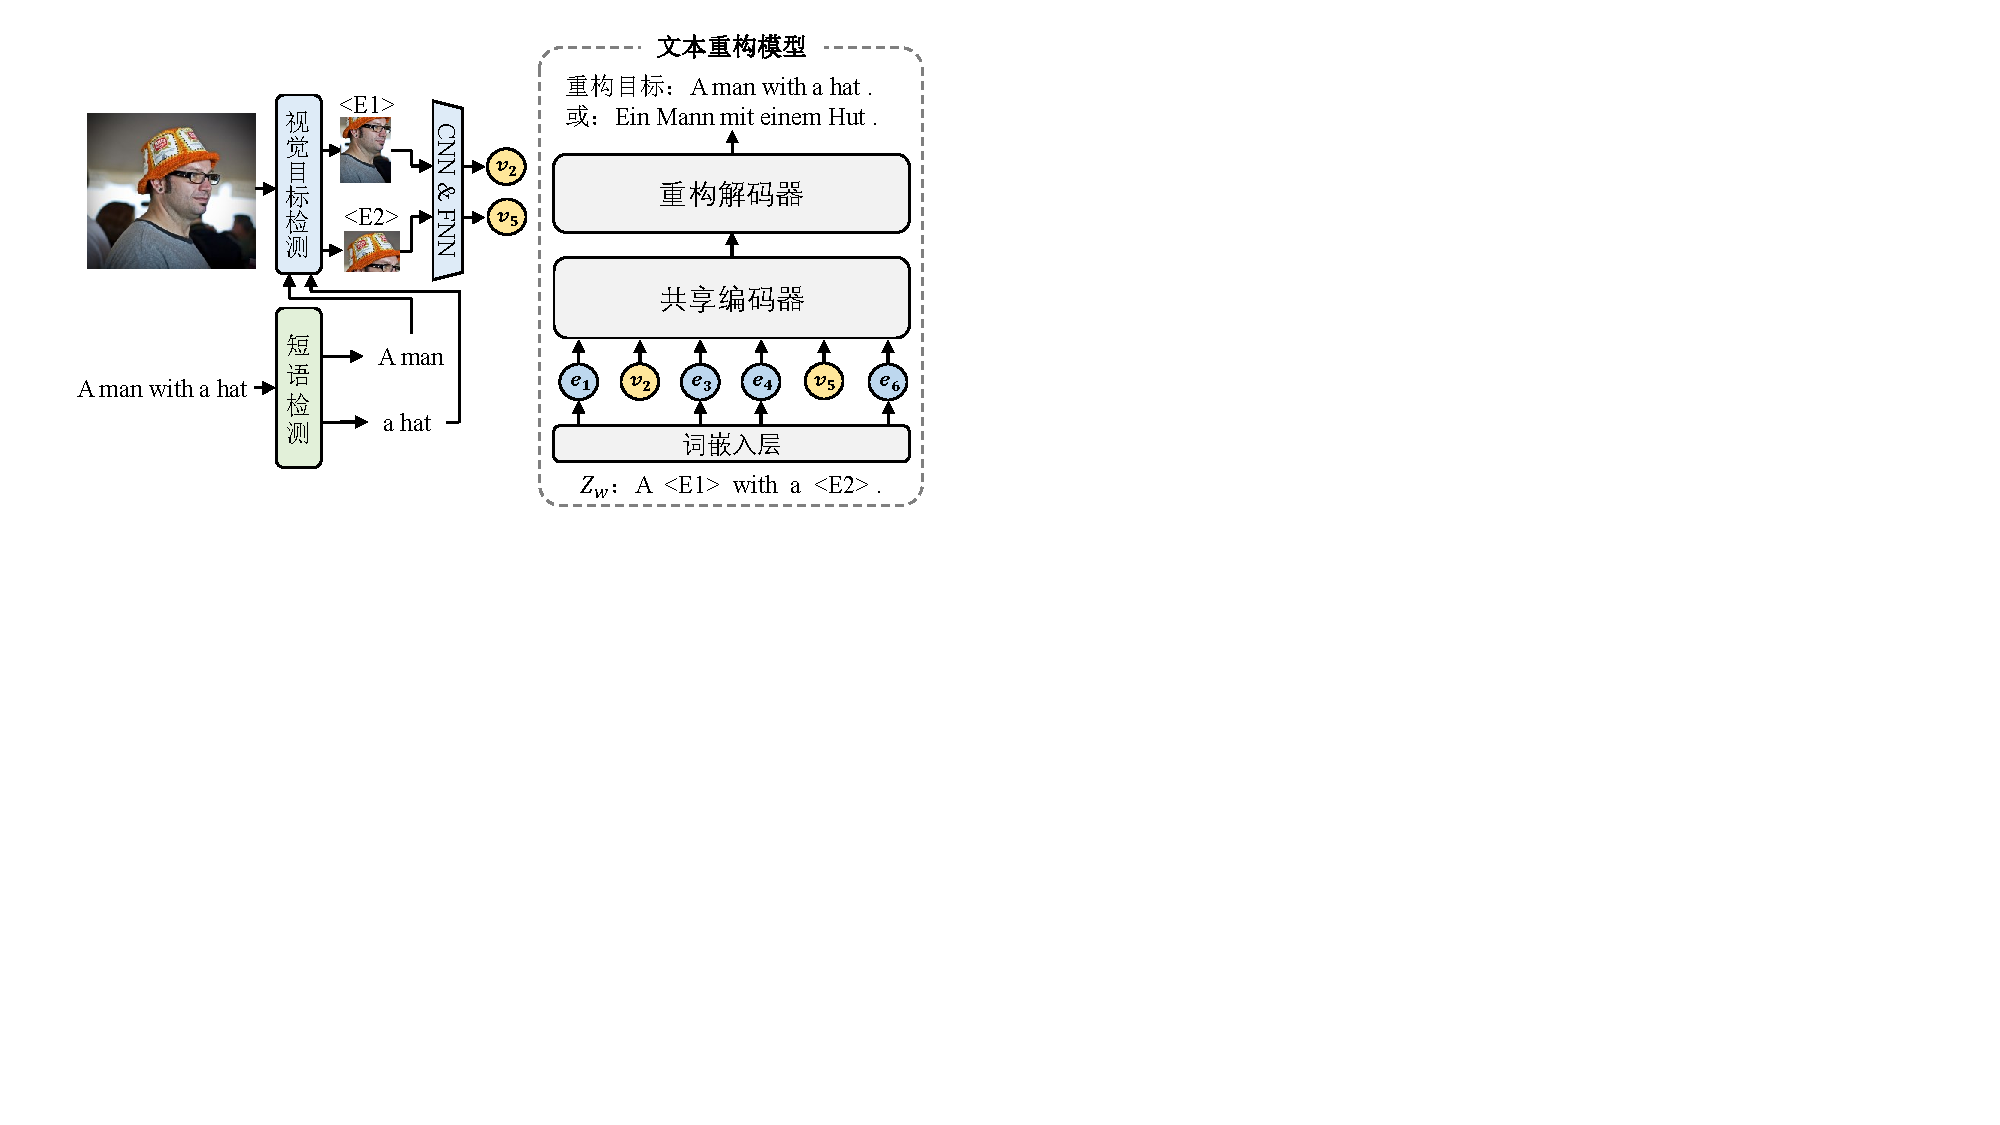
\includegraphics[scale=1.0]{Img/fig_3_reconstruction_model.pdf}
    \bicaption{融合视觉目标信息的文本重构方法}{Text reconstruction by fusing visual object information}
    \label{fig:3_reconstruction_model}
\end{figure}
为了充分融合来自文本模态和视觉模态的信息,本章设计了文本重构模型使显式跨模态信息融合方法有效。如图\ref{fig:3_reconstruction_model}所示,左侧展示的是利用图\ref{fig:3_entity_extraction}中的方法提取出视觉目标后,再通过预训练的卷积神经网络提取得视觉目标的全局特征,并利用一个前馈神经网络(feedforward neural network,FNN)映射到与词向量相同的维度。图\ref{fig:3_reconstruction_model}右侧的 “文本重构模型”是一个与“翻译模型”相似的序列到序列的生成式模型。模型的多模态输入序列$Z_{w}$是利用WRR得到的退化文本与视觉目标图像的混合序列。该序列的向量表示为$\{\Vector{e_1,v_2,e_3,e_4,v_5,e_6}\}$。重构任务负责从$Z_{w}$生成原始文本$X=\{x_1,x_2,…,x_N\}$。模型因此可以分别在编码阶段的视觉特征空间和解码阶段从语言特征空间学习到实体信息。重构模型的训练方式为最小化以下对数似然损失:
\begin{equation}
    \mathcal{L}_R(\theta, \psi)=-\sum_i^N \log p(x_i|x_{<i},Z)
    \label{eq:3_reconstruction_x}
\end{equation}
其中$Z$可以是使用WRR的$Z_{w}$也可以是采用了PRR的$Z_{p}$,$\theta$为重构模型的编码器参数,$\psi$为重构模型的解码器参数。
考虑到重构目标语言$Y=\{y_1,y_2,\cdots,y_M\}$也是一种可行方案。此时,目标函数调整为:
\begin{equation}
    \mathcal{L}_R(\theta, \psi)=-\sum_j^M \log p(y_j|y_{<j},Z)
    \label{eq:3_reconstruction_y}
\end{equation}

\subsection{与机器翻译相结合}
\label{sec:3_multitask}
图\ref{fig:3_reconstruction_model}中所展示的重构模型与一般的神经机器翻译模型相似,都是基于编码器-解码器结构的端到端生成模型。其中翻译模型的目标函数也与公式(\ref{eq:3_reconstruction_x})和公式(\ref{eq:3_reconstruction_y})相近:
\begin{equation}
    \mathcal{L}_T(\theta, \phi)=-\sum_j^M \log p(y_j|y_{<j},X)
    \label{eq:3_translation}
\end{equation}
其中$\phi$为神经翻译模型的解码器参数。为了将重构任务和翻译任务结合,本章按照\tcite{elliott2017imagination}的方式将两者的目标函数结合:
\begin{equation}
    \mathcal{L}(\theta, \psi, \phi)=\omega L_T(\theta, \phi) + (1-\omega)L_R(\theta, \psi)
    \label{eq:3_combine_sr}
\end{equation}
其中$\omega$是调节两个任务训练比例的超参数,即当前批数据(batch)用于更新翻译模型参数的概率。相对应的,用于更新文本重构模型参数的概率为$1-\omega$。当前的多任务学习通过共享编码器参数来达到知识迁移的目的。

\subsection{参数共享策略}
\label{sec:3_parameter_sharing}
% 
\begin{figure}[!htbp]
    \centering
    \begin{subfigure}[b]{0.5\textwidth}
      \centering
      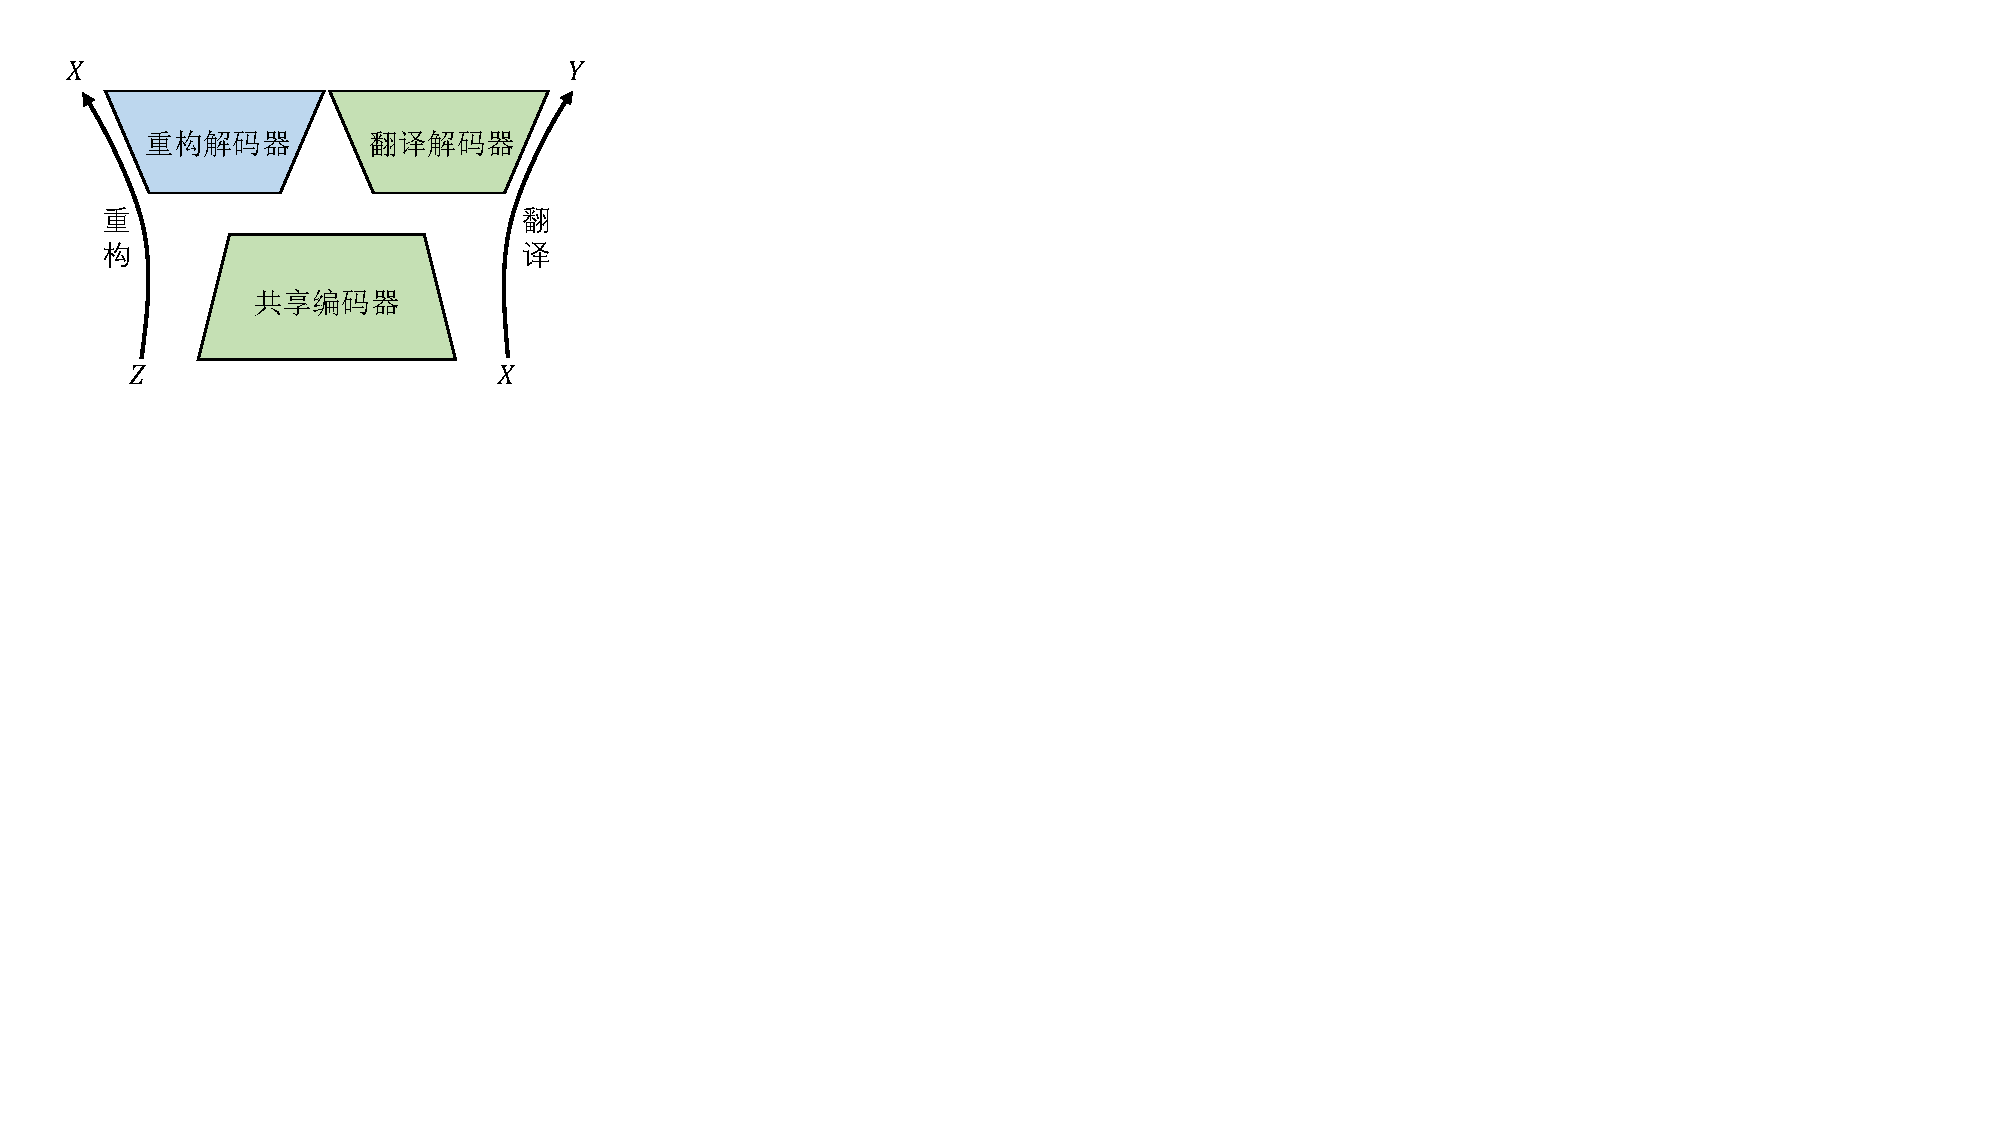
\includegraphics[scale=0.7]{Img/fig_3_sr.pdf}
      \caption{源-独享}
      \label{fig:3_sr}
    \end{subfigure}%
    ~% add desired spacing
    \begin{subfigure}[b]{0.5\textwidth}
      \centering
      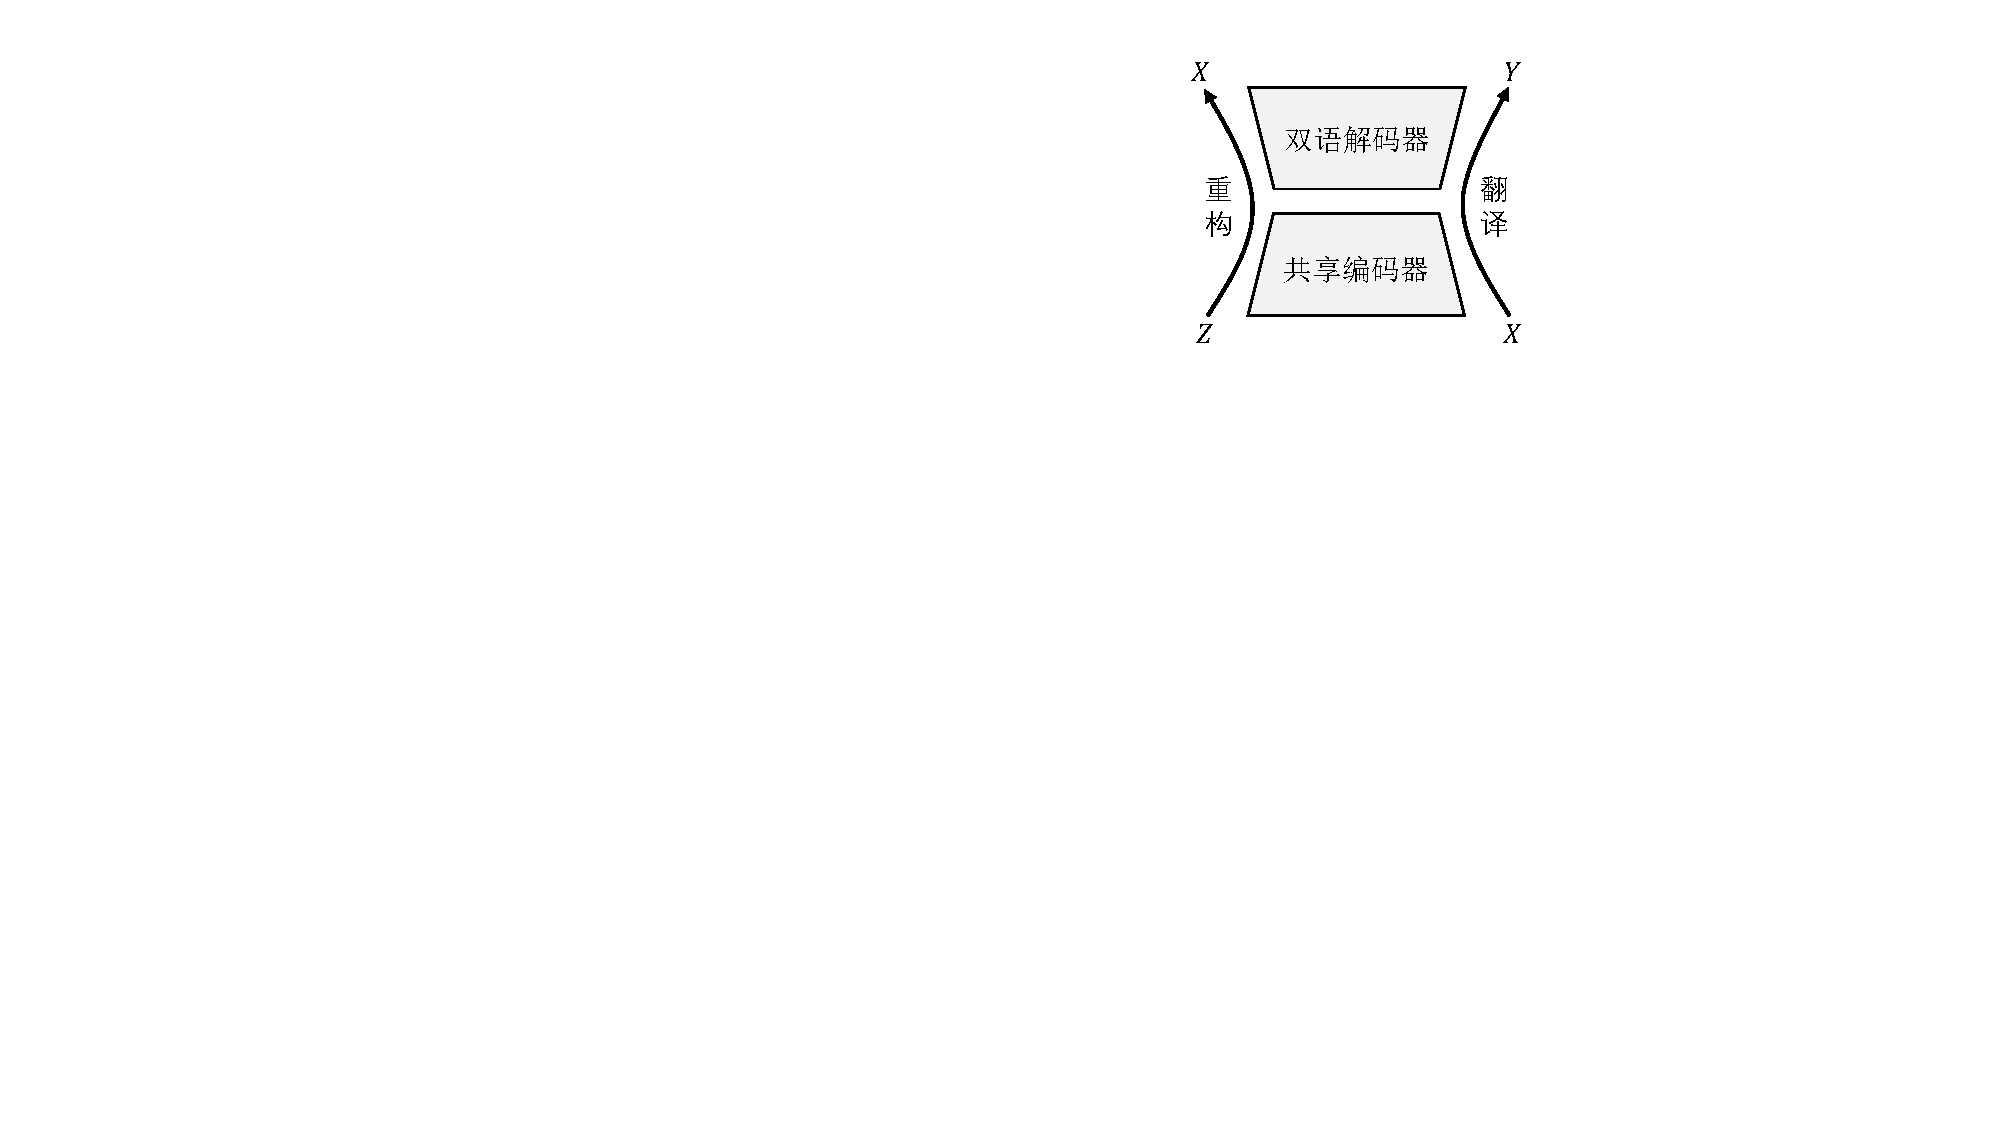
\includegraphics[scale=0.7]{Img/fig_3_ss.pdf}
      \caption{源-共享}
      \label{fig:3_ss}
    \end{subfigure}
    \\% line break
    \begin{subfigure}[b]{0.5\textwidth}
      \centering
      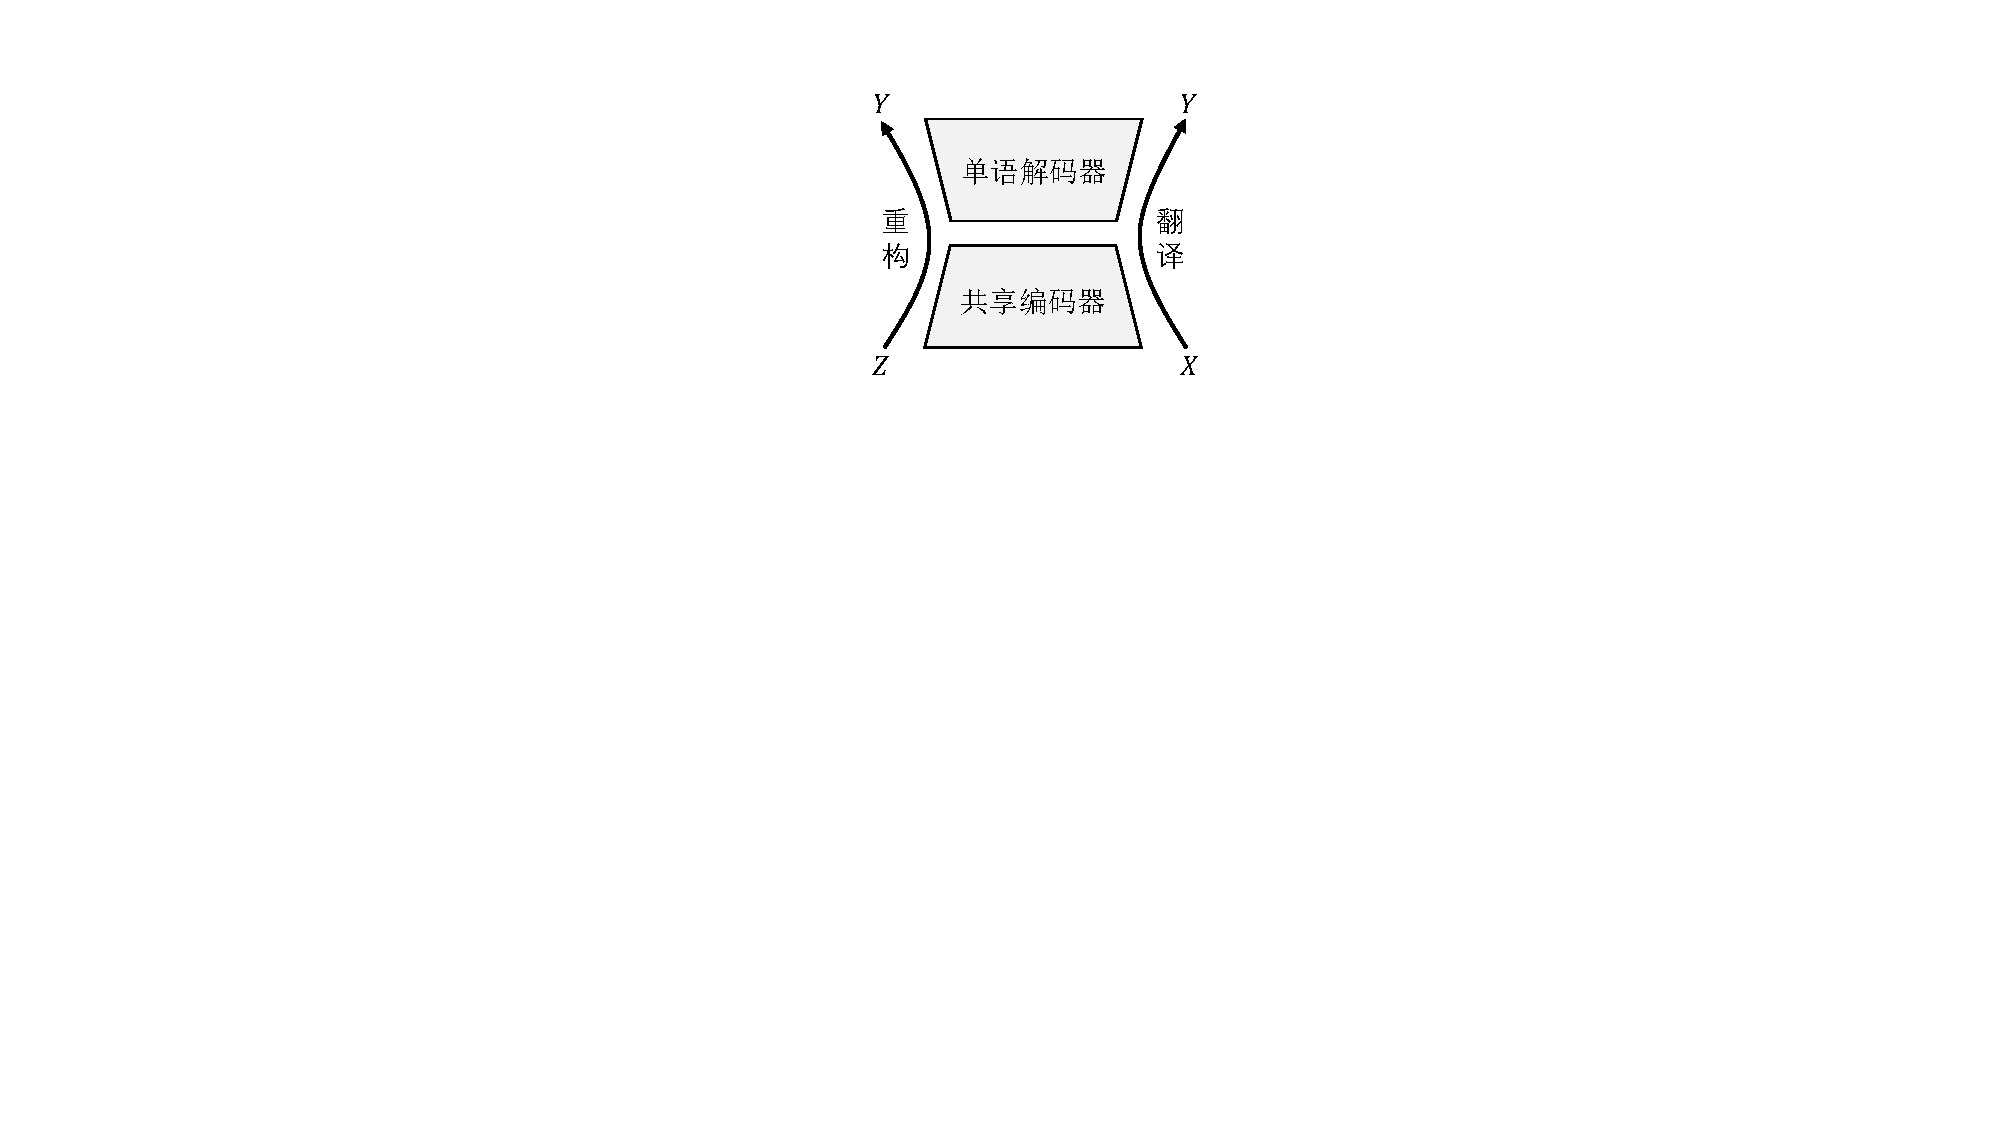
\includegraphics[scale=0.7]{Img/fig_3_t.pdf}
      \caption{目-共享}
      \label{fig:3_t}
    \end{subfigure}%
    \bicaption{重构模型与翻译模型的参数共享方案}{Parameter sharing schemes between reconstruction model and translation model}
    \label{fig:4_fidelity}
\end{figure}
正如前面章节所提到,重构模型与翻译模型在结构上有高度的相似性,因此可以利用参数共享的方法将重构模型学习到的视觉信息融合到翻译模型中,从而达到提升翻译质量的目的。因此,由编码器-解码器结构的灵活性与两种重构目标可组合得到多种参数共享方案。本文采用了以下三种参数共享方案。

(1){\sffamily 独享解码器重构源语言}
\begin{figure}[!htbp]
    \centering
    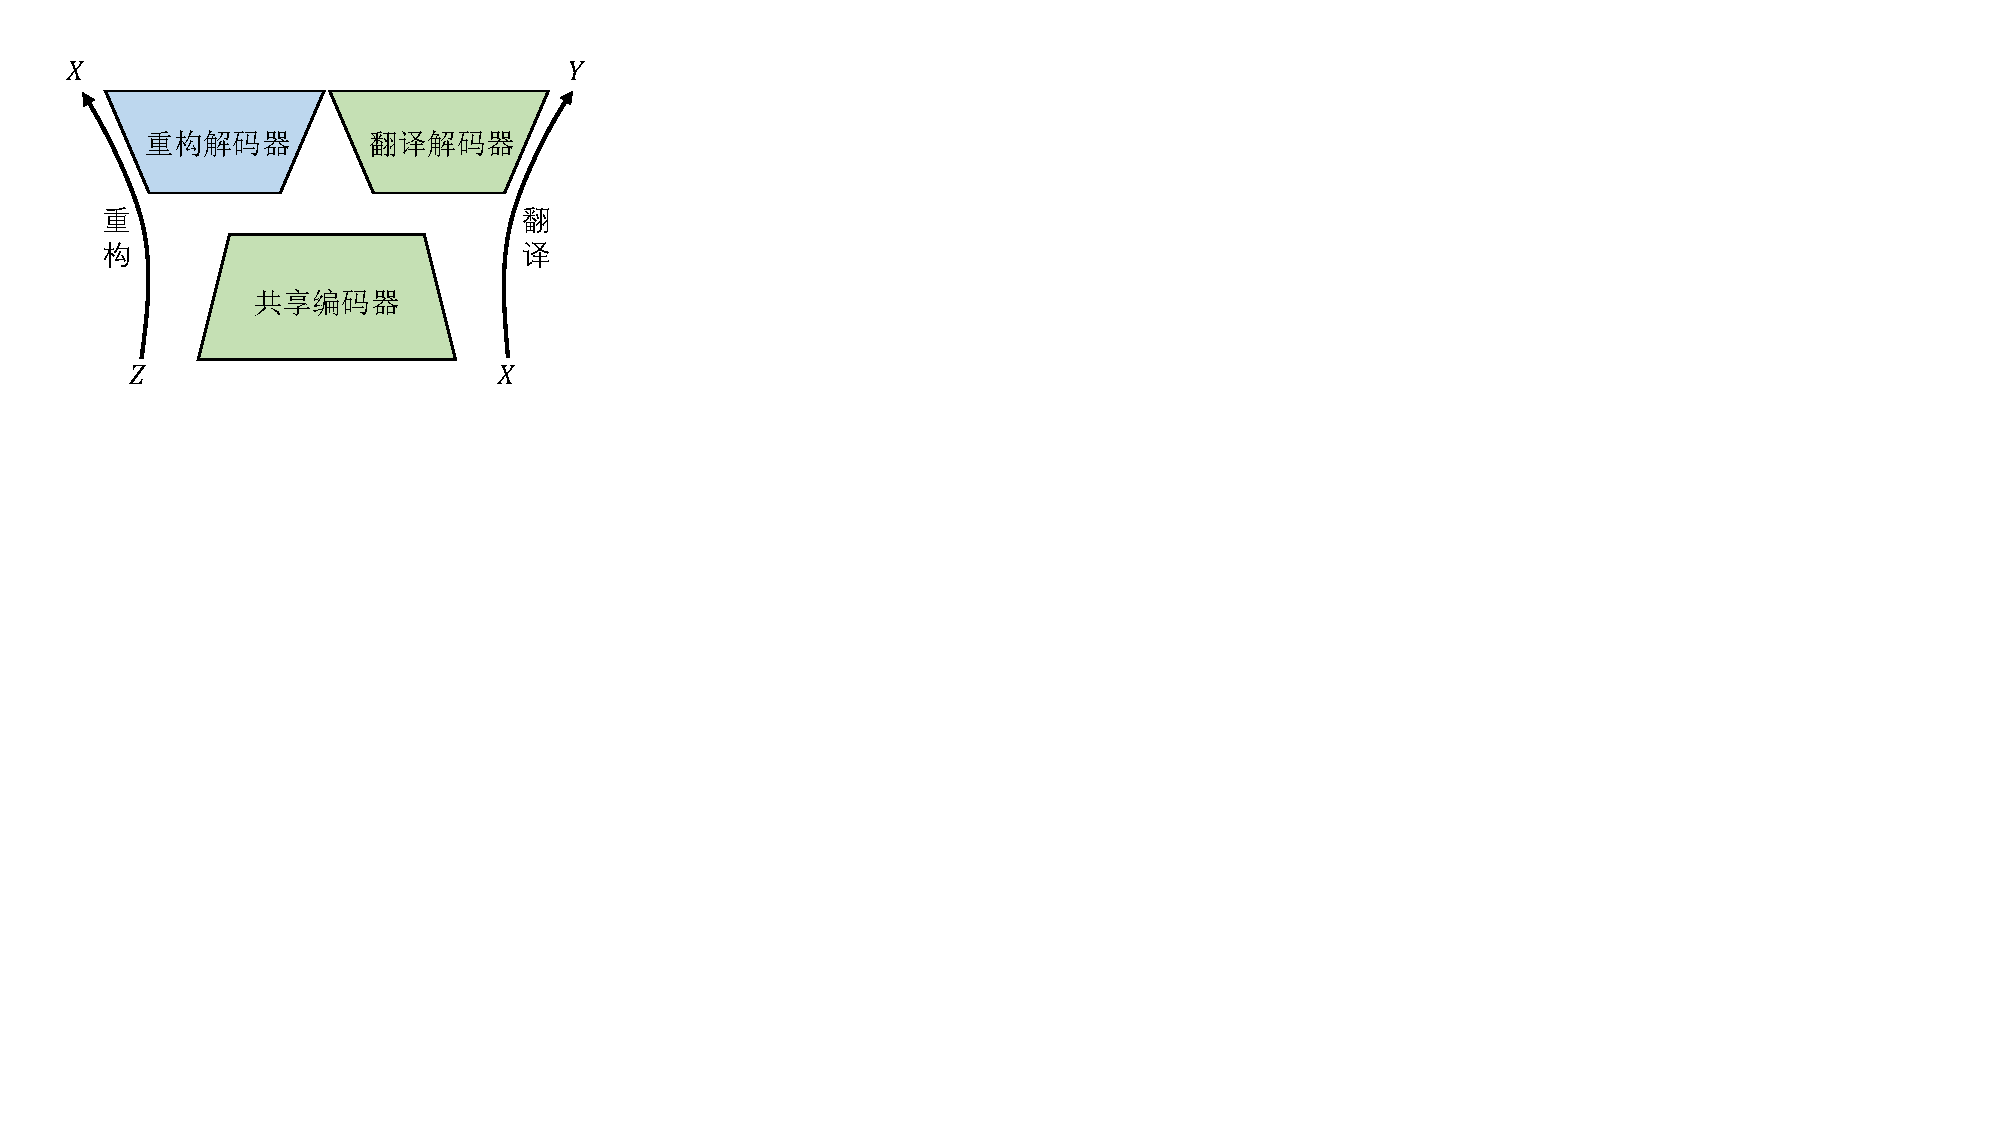
\includegraphics[scale=0.9]{Img/fig_3_sr.pdf}
    \bicaption{独享解码器重构源语言“源-独享”}{Reconstruction for source language with respective decoder}
    \label{fig:3_sr}
\end{figure}

由于视觉信息要在编码的过程中学习特征表示,因此在所有的参数共享策略中,都要包含共享编码器。解码器的参数共享则是可选的。在利用独享解码器重构源语言的策略中,为源语言和目标语言设立独立的解码器,即重构模型和翻译模型的编码器是共享的,解码器参数是独享的。联合目标函数为公式(\ref{eq:3_combine_sr}),在后面的实验中,本文用“源-独享”表示应用该策略。

(2){\sffamily 共享解码器重构源语言}
\begin{figure}[!htbp]
    \centering
    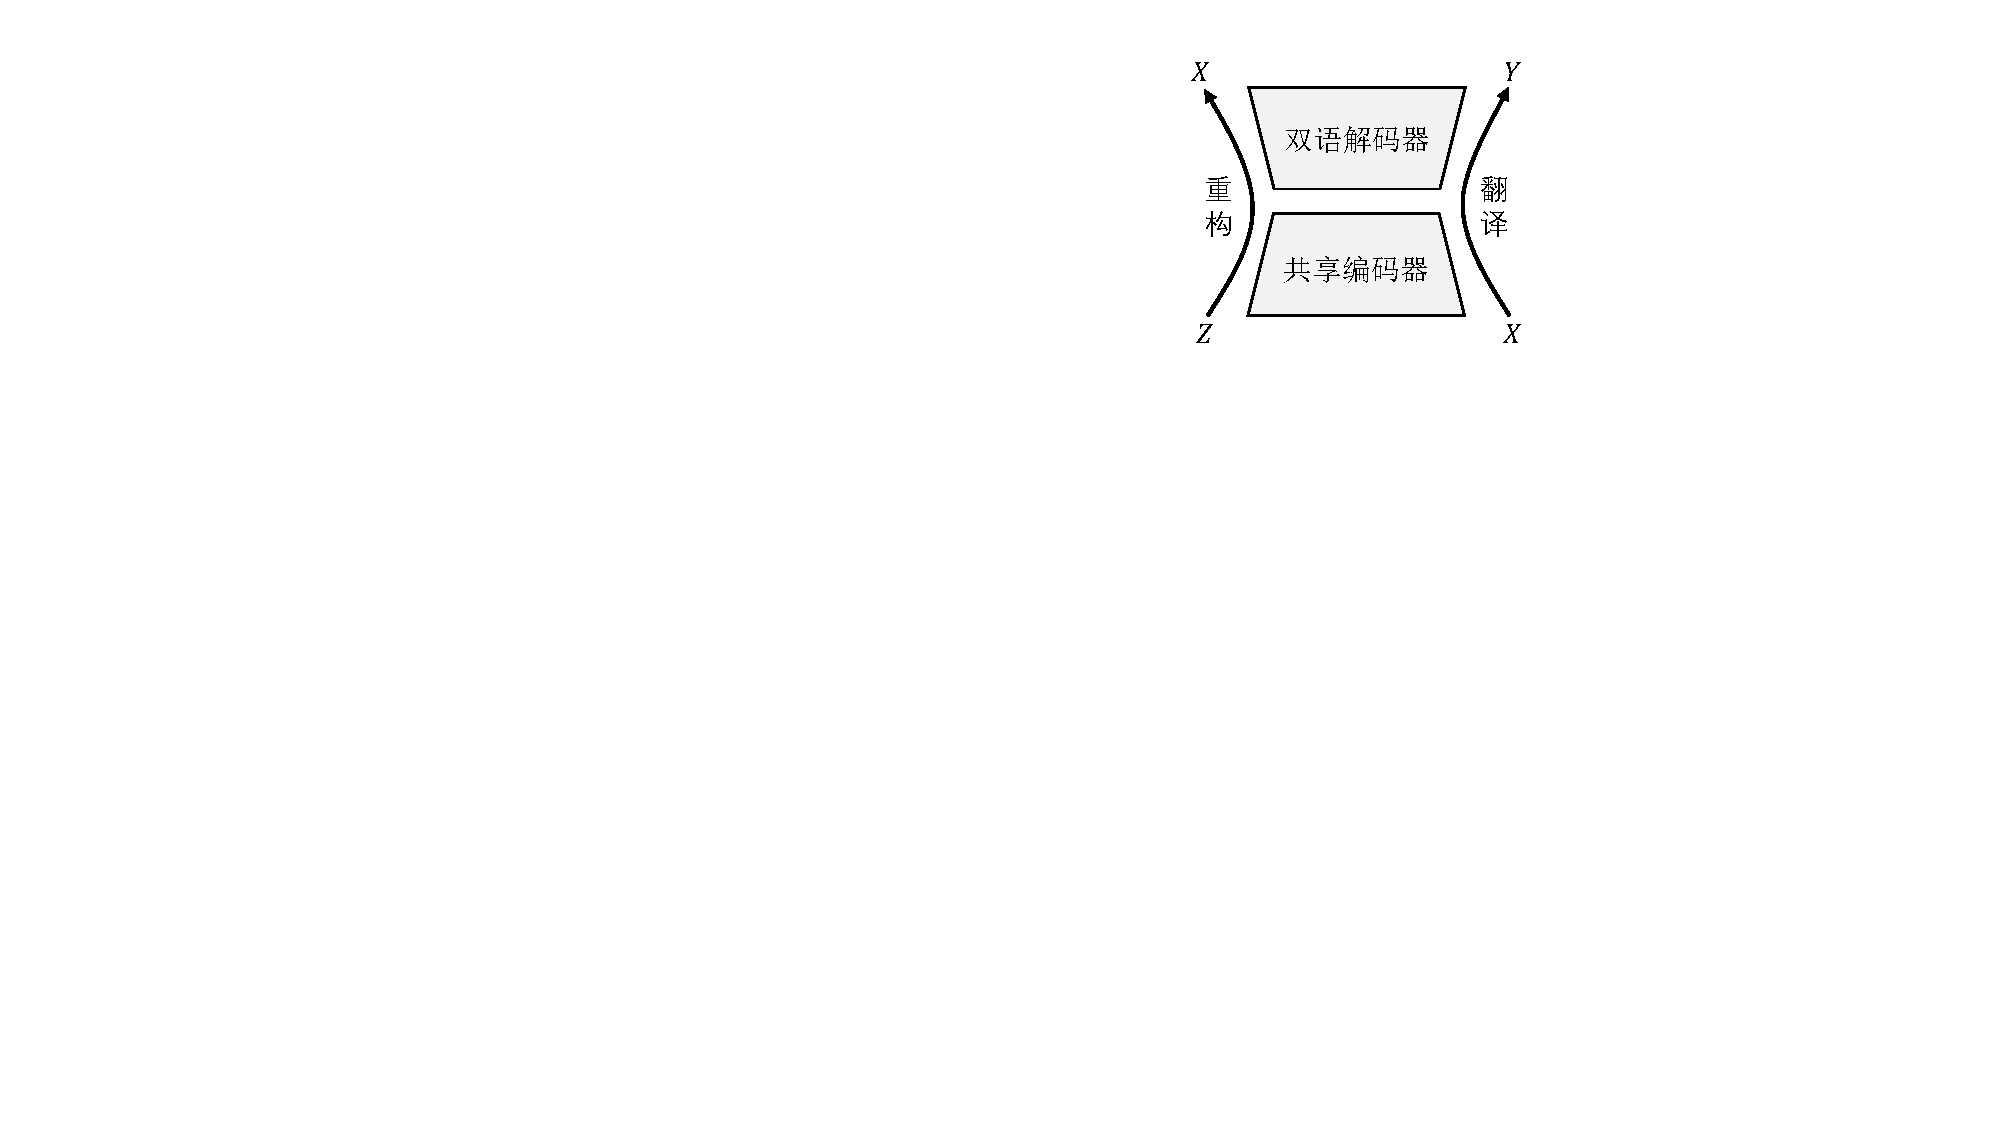
\includegraphics[scale=1]{Img/fig_3_ss.pdf}
    \bicaption{共享解码器重构源语言“源-共享”}{Reconstruction for source language with shared decoder}
    \label{fig:3_ss}
\end{figure}

通过融合源语言和目标语言的词表,以及在编码器和解码器之间共享词嵌入层的方式,可以实现重构模型和翻译模型的共享解码器的设置。同时,需要在解码过程中,目标语言句子在解码端的输入需要在句首引入一个“识别词”(例如,“<en\_sos>”表示解码到英语,“<de\_sos>”表示解码到德语)用于表示当前解码器用于重构到源语言还是翻译到目标语言。在该设置中,对于公式(\ref{eq:3_combine_sr})有$\psi=\phi$。这表明该策略中翻译模型和重构模型是全参数共享的。因此,将联合目标函数调整为:
\begin{equation}
    \mathcal{L}(\theta, \phi)=\omega \mathcal{L}_T(\theta, \phi) + (1-\omega)\mathcal{L}_R(\theta, \phi)
    \label{eq:3_combine_ss}
\end{equation}
本文将用“源-共享”代表该参数共享策略。

(3){\sffamily 共享解码器重构目标语言}
\begin{figure}[!htbp]
    \centering
    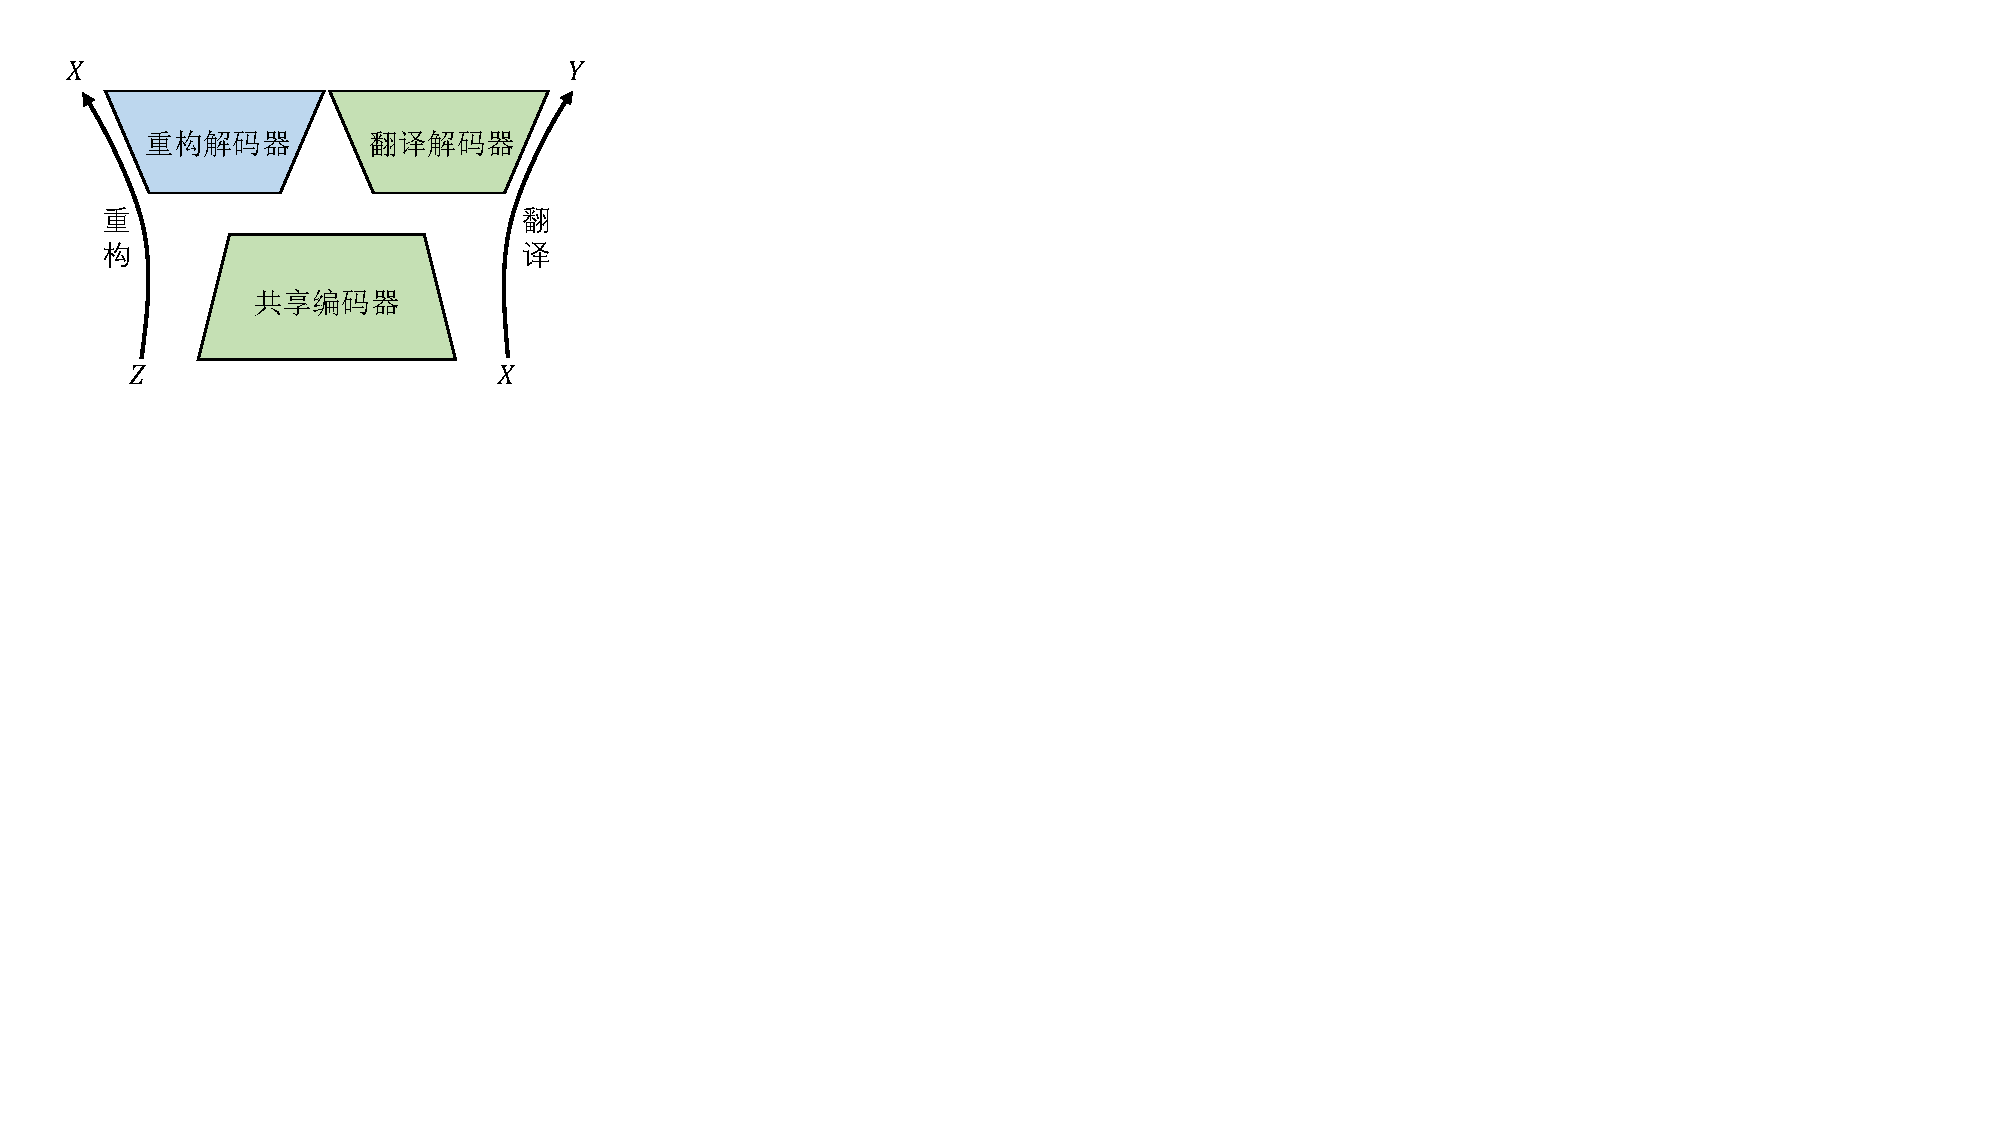
\includegraphics[scale=0.9]{Img/fig_3_sr.pdf}
    \bicaption{共享解码器重构目标语言“目-共享”}{Reconstruction for target language with shared decoder}
    \label{fig:3_t}
\end{figure}

不同于重构源语言,解码器的参数共享策略在重建目标语言的方向上则很容易实现。在该策略中,重构任务的工作方式与一般的ImgNMT模型相似,区别在于输入的文本是文本信息不完整的退化文本。并且其联合目标函数与公式(\ref{eq:3_combine_ss})相同。本文将用“目-共享”来表示该参数共享策略。
\section{实验设置}
为了验证所提方法的有效性,本章在基于循环神经网络和基于Transformer的两种模型上进行了测试。本章选择了融合图片信息的神经机器翻译中最常用的Multi30K\pcite{elliott2016multi30k}数据集的英德翻译进行实验。

\subsection{实验数据}
本文使用图像描述翻译的Multi30K翻译数据集英德翻译对。该数据集每张图片配有一个英文句子和与其对应的德文翻译。该数据集共包含31014张图片,并划分为训练集、验证集和测试集三部分,对应的图片数量分别为:29000,1014和1000。另外,本章还采用了WMT17发布的测试集,包含Multi30K 2017测试集和针对歧义词的ambiguous MSCOCO 2017测试集。这两个测试集同样是每张图片配有一个英文句子和德文翻译,对应的图片数量分别为:1000和461。本文采用Moses SMT\pcite{koehn2007moses}(byte pair encoding, BPE)或WordPiece\pcite{wu2016google}进行分词操作。经过以上预处理后,得到英文词表大小为10209,德文词表为18674,合并后的双语词表大小为27226。

\subsection{实体提取}
\label{sec:3_setup_entity_extraction}
实体提取采用的是\ref{sec:3_entity_extraction}节介绍的方法。其中名词和名词短语提取模块采用的是spaCy\footnote{https://spacy.io/}提供的提取名词短语和词性标注功能。在采用词级替换规则时,所替换的名词占训练集和测试集单词统计量的32.6\%。采用短语级替换规则时,提取的名词短语占单词统计量的45.1\%。同时,我们观察了在词级和短语级替换规则中,所涉及单词的词频情况。两种替换规则下,所涉及单词的词频中位数都是2,这意味着这些词中多数都是低频词。提前视觉目标采用的是\tcite{yang2019a}所提方法。理论上,只有实体短语可以从图片中检测到,没有在图片中检测到对应视觉目标的名词短语不被列为短语实体。另一种得到对齐的名词短语与视觉目标的方法是使用已标注的数据,Flickr30K Entities\pcite{plummer2015flickr30k,plummer2017flickr30k}就是标注了图片与文本中实体对应关系的数据集。该数据集与Multi30K高度重合,因此可以直接利用到本章所提方法上。对于从图片中截取到的视觉目标图片,本章利用在ImageNet\pcite{russakovsky2015imagenet}上预训练的ResNet-50\pcite{he2016deep}提取2048维的全局特征。

\subsection{基于循环神经网络的模型设置}
\label{sec:3_rnn_setup}
对于基于循环神经网络的翻译模型,本章采用的是带有注意力机制并基于编码器-解码器结构的神经翻译模型\pcite{luong2015effective}。其中,编码器是一个维度维500的单层双向的LSTM,重构模型和翻译模型的解码器都是单层500维的LSTM,词嵌入层的维度同样设置为500。编码器和解码器中的dropout均设置为0.3。模型参数是从$(-0.1,+0.1)$区间的均匀分布中采样初始化的,其中偏置项(bias)初始化为0。训练时采用Adam\pcite{kingma2014adam}优化器优化模型参数,学习率设为定值0.002。批数据大小(batch size)为40。最终模型是根据验证集在BLEU4\pcite{papineni2002bleu}上的表现进行选择。在训练过程中,当模型在验证集上的BLEU4值超过10个迭代轮次不再提升,则停止训练并作为最终用于评测的模型。

\subsection{基于Transformer的模型设置}
\label{sec:3_transformer_setup}
对于基于Transformer\pcite{vaswani2017attention}的翻译模型,本章将词向量的维度设置为128,隐层状态维度设置为256,自注意力的头数为4,模型编码器和解码器的层数均为4,dropout设置为0.2,批数据大小为2000个单词。区别于基于RNN的模型,Transformer采用的是合并的词表,因此词表大小始终设置为合并词表的大小27226。模型优化采用的是Adam优化器,其中$\beta_1=0.9$,$\beta_2=0.998$,$\epsilon=10^{-9}$。本章与\tcite{vaswani2017attention}相同采用预热和衰减策略来提高学习率,预热步骤为4000,总训练步骤为80000。训练目标中设置平滑标签(label smoothing)$\epsilon_{ls}=0.1$。测试时,采用了搜索空间$b=4$的柱搜索算法。以上模型参数与\tcite{yin2020novel}中的模型设置基本一致。

\subsection{多任务训练}
本章所提方法需要对重建任务和翻译任务采用多任务训练的方式进行模型优化。多任务训练采用的是两个任务随机交替训练的方式,并利用\ref{sec:3_multitask}节中所介绍的超参数$\omega$控制翻译任务的训练概率。因为两个任务所使用数据的比例相同,因此本章设置$\omega=0.5$。

\subsection{对比模型}
基于循环神经网络的模型:
\begin{itemize}
    \item \textbf{NMT:}基于LSTM的纯文本神经翻译模型,其模型配置与\ref{sec:3_rnn_setup}节中的描述保持一致。
    \item \textbf{pRCNNs\pcite{huang2016attention}:}该模型在编码阶段将每个视觉目标特征与源语言句子编码一次,在解码阶段,解码器选择关注与当前解码步骤相关的视觉目标所对应的文本序列。
    \item \textbf{DATT\pcite{calixto2017doubly}:}该模型设置了两个注意力机制模块,其中一个用于关注文本信息,另一个用于关注图片的栅格特征。并设置了一个门控值控制图片信息输入的量。
    \item \textbf{Imagination\pcite{elliott2017imagination}:}该方法将源语言句子编码后,利用编码后的隐层表示预测输入句子所对应的图片。该方法同样使用了多任务的方式。
    \item \textbf{VMMT\pcite{calixto2019latent}:}该方法中的$ \mathrm{VMMT_C} $与$ \mathrm{VMMT_F} $采用隐变量建模语义信息,在翻译过程中利用视觉信息与文本信息使变分编码器融合跨模态语义。
\end{itemize}

基于Transformer的模型:
\begin{itemize}
    \item \textbf{Transformer:}基于Transformer的纯文本神经机器翻译模型,其模型配置与\ref{sec:3_transformer_setup}节保持一致。
    \item \textbf{DelMMT\pcite{ive2019distilling}:}该模型提出使用推敲做多模态二次接码。在二次解码中融合源语言、目标语言以及视觉信息。
    \item \textbf{MMT-TF\pcite{yao2020multimodal}:}该工作设计了一种多模态注意力模块,该模块需要链接源语言句子的表示和图像特征作为自注意力模块的查询。
    \item \textbf{GAMMT\pcite{liu2021gumbel}:}使用Gumbel-Sigmoid改造注意力机制,帮助翻译模型关注到图片中与文本内容更相关的区域。
    \item \textbf{GMMT\pcite{yin2020novel}:}该模型视源语言句子与图片中的视觉目标为一个多模态图结构,然后利用设计的基于图的跨模态编码器进行编码,最终解码出目标端句子。
\end{itemize}

\section{实验结果}

\subsection{英德翻译结果}

\begin{table}[!htbp]
    \bicaption{基于RNN的神经翻译模型在Multi30K数据集英译德翻译方向的实验结果}{Experiment results of RNN-based NMT on the Multi30K En-De translation pair.}
    \label{tab:3_rnn_ende}
    \centering
    \footnotesize% fontsize
    \setlength{\tabcolsep}{4pt}% column separation
    \renewcommand{\arraystretch}{1.2}%row space 
    \begin{tabular}{cccccccc}
        \hline
        \multicolumn{2}{c}{\multirow{2}{*}{基于RNN}} & \multicolumn{2}{c}{Test2016} & \multicolumn{2}{c}{Test2017} & \multicolumn{2}{c}{MSCOCO} \\ \cline{3-8}
                  & & BLEU        & METEOR      & BLEU         & METEOR        & BLEU         & METEOR   \\ %\hline
    \hline
    \multicolumn{2}{c}{NMT}                                                 & 35.9  & 54.9   & 28.8   & 49.5   & 25.9   & 45.7  \\ %\hline
    \hline
    \multicolumn{2}{c}{pRCNNs \cite{35_huang-etal-2016-attention}}             & 36.5   & 54.1   & -           & -           & -           & -           \\
    \multicolumn{2}{c}{DATT \cite{36_calixto-etal-2017-doubly}}                & 36.5        & 55.0        & -           & -           & -           & -           \\
    \multicolumn{2}{c}{Imagination \cite{37_elliott-kadar-2017-imagination}}   & 36.8   & 55.8   & -           & -           & -           & -           \\
    \multicolumn{2}{c}{$ \mathrm{VMMT_C} $ \cite{38_calixto-etal-2019-latent}} & 37.5   & 55.7   & 26.1   & 45.4   & 21.8   & 41.2   \\
    \multicolumn{2}{c}{$ \mathrm{VMMT_F} $ \cite{38_calixto-etal-2019-latent}} & 37.7   & 56.0   & 30.0   & 49.9   & 25.5   & 44.8   \\ \hline%\hline
                      
    \multirow{3}*{词级} & 
       独享-源   & 37.8           & 56.1           & 30.1           & \textbf{50.3}  & \textbf{27.0}  & \textbf{46.4}  \\
     & 共享-源   & \textbf{38.0}  & 56.2           & 30.3           & 50.1           & 26.1           & 45.6  \\
     & 共享-目    & 36.3           & 55.0           & 28.4           & 48.6           & 25.3           & 44.3  \\ %\hline
    \hline
    \multirow{3}*{短语级} & 
        独享-源  & \textbf{38.0}  & \textbf{56.5}  & 30.2           & \textbf{50.3}  & 26.8           & 46.1  \\
     &  共享-源  & 37.8           & 56.1           & \textbf{30.5}  & 50.1           & 26.0           & 45.5  \\
     &  共享-目  & 36.8           & 55.0           & 29.4           & 49.0           & 26.3           & 45.3  \\ 
        \hline
    \end{tabular}
\end{table}
如\ref{sec:3_entity_replacement}和\ref{sec:3_parameter_sharing}节所述,本章共设置了两种实体替换规则:短语级和词级,以及三种模型参数共享策略:独享解码器重构源语言、共享解码器重构源语言以及共享解码器重构目标语言,并分别以“独享-源”、“共享-源”和“共享-目”作为简化表示,对以上实验配置进行组合后共得到6种模型设置方案。另外,本章还针对以上设置在基于RNN和基于Transformer的机器翻译模型上都进行了实验,并在BLEU\pcite{papineni2002bleu}和Meteor\pcite{denkowski2014meteor}两个指标上进行比较。

{\sffamily 基于RNN的模型实验结果:}表\ref{tab:3_rnn_ende}展示了采用基于RNN的神经机器翻译模型在英译德翻译对上的实验结果,其中加粗项表示同列中最好的实验结果。本章与5个融合图片信息的神经机器翻译方法进行了对比,其中pRCNNs和DATT需要在测试过程中为模型输入图片,其它模型包括本章所设计的翻译模型在测试阶段不需要输入图片。该实验结果展示了本章所提方法在纯文本翻译的基础上得到了显著的提升,表明了我们的方法在基于RNN的模型上的有效性。该实验结果同样显示出了6中实验方案的优缺点。对于重构到源语言句子,实验结果中没有表现出采用共享解码器或独享解码器两种配置之间的明显差距,同样在采用词级替换规则或是短语级替换规则的差别也不大。对于重构到目标语言句子,可以观察到其实验结果明显的低于重构到源语言的方案。以上信息表明,为重构任务设置的语言方向是影响本章所提方法实验效果的最大因素。


\begin{table}[!htbp]
    \bicaption{基于Transformer的神经翻译模型在Multi30K数据集上的实验结果}{Experiment results of Transformer-based NMT on the Multi30K dataset.}
    \label{tab:3_transformer_ende}
    \centering
    \footnotesize% fontsize
    \setlength{\tabcolsep}{4pt}% column separation
    \renewcommand{\arraystretch}{1.2}%row space 
    \begin{tabular}{lccccccc}
        \hline
        \multicolumn{2}{c}{\multirow{2}{*}{基于Transformer}} & \multicolumn{2}{c}{Test2016} & \multicolumn{2}{c}{Test2017} & \multicolumn{2}{c}{MSCOCO} \\ \cline{3-8}
                  & & BLEU        & Meteor      & BLEU         & Meteor        & BLEU         & Meteor   \\ %\hline
    \hline
    \multicolumn{2}{l}{~~~~Transformer}                                     & 38.5       & 57.5      & 31.0   & 51.9   & 27.5   & 47.4     \\\hline
    \multicolumn{2}{l}{~~~~DelMMT \pcite{ive2019distilling}}          & 38.0            & 55.6           & -           & -           & -           & -             \\
    \multicolumn{2}{l}{~~~~MMT-TF \pcite{yao2020multimodal}}           & 38.7            & 55.7           & -           & -           & -           & -             \\
    \multicolumn{2}{l}{~~~~GAMMT \pcite{liu2021gumbel}}  & 39.2            & \textbf{57.8}  & 31.4        & 51.2        & 26.9        & 46.0          \\
    \multicolumn{2}{l}{~~~~GMMT \pcite{yin2020novel}}                 & \textbf{39.8}   & 57.6           & 32.2        & 51.9        & 28.7        & \textbf{47.6} \\ \hline%\hline
    \multicolumn{8}{c}{CTR-NMT}\\\hline
    \multirow{3}*{~~词级} & 
       独享-源   & 39.7       & 57.5             & \textbf{32.9}    & 51.7             & \textbf{29.1}    & 47.5   \\
     & 共享-源   & 39.4       & \textbf{57.8}    & 32.4             & \textbf{52.1}    & 28.3             & 47.5   \\
     & 共享-目   & 38.7       & 56.2             & 31.0             & 49.6             & 26.5             & 44.9     \\ %\hline
    \hline
    \multirow{3}*{~~短语级} & 
        独享-源  & 39.3       & 57.4             & 32.7             & 51.8             & 28.7             & 47.5   \\
     &  共享-源  & 39.0       & 57.3             & 32.4             & 51.6             & 28.3             & 47.2   \\
     &  共享-目  & 38.5       & 56.2             & 30.5             & 49.7             & 26.8             & 45.6   \\
        \hline
    \end{tabular}
\end{table}
{\sffamily 基于Transformer的模型实验结果:}表\ref{tab:3_transformer_ende}展示了采用基于Transformer的神经机器翻译模型在英译德翻译对上的实验结果,其中加粗项表示同列中最好的实验结果。5个对比模型中,仅Transformer为纯文本神经机器翻译方法,其它4个模型均需要在测试阶段输入图片。而本章所提方法仅需要在训练阶段输入图片,在测试阶段并不需要。从模型结果的比较中可以观察到,本章所提方法能够有效地提升纯文本神经翻译模型的翻译准确率,在测试阶段没有输入图片的劣势情况下,本章所提方法依旧与其它方法是可比的。另外,在基于6种模型设置方案的结果比较中可以观察到与基于RNN的模型有相似的现象,即重构的语言方向是影响方法性能的主要因素。该实验结果中还可以发现,词级替换规则的实验结果略优于短语级。


% Table generated by Excel2LaTeX from sheet 'flickr'
\begin{table}[!htbp]
    \bicaption{基于Flickr30K Entities标注实体的实验结果}{Experiment results on the annotated entities provided by Flickr30K entities}
    \label{tab:3_flickr30k_entities}
    \centering
    \footnotesize% fontsize
    \setlength{\tabcolsep}{4pt}% column separation
    \renewcommand{\arraystretch}{1.2}%row space 
    \begin{tabular}{clcccccccc}
    \hline
    \multicolumn{2}{c}{\multirow{2}{*}{模型}} & \multicolumn{4}{c}{基于RNN} & \multicolumn{4}{c}{基于Transformer} \\ \cline{3-10}
    & & \multicolumn{2}{c}{BLEU} & \multicolumn{2}{c}{METEOR} & \multicolumn{2}{c}{BLEU} & \multicolumn{2}{c}{METEOR} \\\hline

    \multirow{3}*{词级} & 
       独享-源   & \textbf{38.0}  & {$\uparrow$ 0.2}  & 56.1  & - 0.0           &  \textbf{39.9}  & {$\uparrow$ 0.2}  & \textbf{58.0}  & {$\uparrow$ 0.3}\\
     & 共享-源   & 38.0  & - 0.0                                    & 55.9  & {$\downarrow$ 0.3}           &  \textbf{39.5}  & {$\uparrow$ 0.1}  & 57.2   & {$\downarrow$ 0.6}        \\
     & 共享-目    & \textbf{36.7}  & {$\uparrow$ 0.4}  & \textbf{55.5}  & {$\uparrow$ 0.5}  &  38.0  & {$\downarrow$ 0.7}           & \textbf{56.9}  & {$\uparrow$ 0.7}\\ \hline
    \multirow{3}*{短语级} & 
       独享-源   & \textbf{38.1}  & {$\uparrow$ 0.1}  & \textbf{56.6}  & {$\uparrow$ 0.1}  &  \textbf{39.4}  & {$\uparrow$ 0.1}  & 57.3   & {$\downarrow$ 0.1}        \\
     & 共享-源   & 37.8  & - 0.0                                    & \textbf{56.2}  & {$\uparrow$ 0.1}  &  \textbf{39.3}  & {$\uparrow$ 0.3}  & 57.1   & {$\downarrow$ 0.2}        \\
     & 共享-目    & \textbf{36.9}  & {$\uparrow$ 0.1}  & \textbf{55.3}  & {$\uparrow$ 0.3}  &  \textbf{38.8}  & {$\uparrow$ 0.3}  & \textbf{56.6}  & {$\uparrow$ 0.4}\\ 
    \hline
    \end{tabular}%
\end{table}%
{\sffamily 基于标注实体的实验结果:}Flickr30K Entities数据集为Multi30K数据集标注了句子中名词短语与图片中视觉目标的对应关系。因此,为了将这些标注数据应用到本章的方法中,仅需要利用词性标注工具识别出这些短语中的名词。表\ref{tab:3_flickr30k_entities}为应用Flickr30K Entities在基于RNN和基于Transformer的模型上的实验结果。加粗项表示相比于表\ref{tab:3_rnn_ende}和表\ref{tab:3_transformer_ende}中相同模型配置下有翻译准确率提升的实验结果。可以观察到,在应用了标注数据后,多数模型都得到了少许翻译准确率的提升。此外还可以观察到,“独享-源”的实验结果普遍要略好于“共享-源”,即重构任务和翻译任务采用各自单独的解码器时效果更佳。

综合以上结果,词级替换规则略优于短语级,应用单独的解码器略优于共享解码器,重构的语言方向影响最大,重构源语言句子带来的翻译准确率提升最多。

\subsection{对抗评估与消融实验}
\label{sec:3_adversarial_ablation}

\tcite{elliott2018adversarial}指出,存在部分融合图片信息的神经机器翻译方法所获得的翻译准确率提升与输入的视觉信息相关性不大。在对这部分模型的输入图像进行随机替换后,模型翻译准确率没有表现出显著的变化。因此,检验视觉信息是否在翻译模型中起了作用对于本章所提方法是一个必要的过程。可根据本章所提方法的结构,假设方法所带来的增益来源于视觉目标中的视觉信息,多任务学习策略,以及模型的抗噪声能力。为此,设计了以下实验来验证方法的有效性:

(1){\sffamily 噪声输入:}在该方案中,本文应用两种噪声输入方法:随机图片和随机单词。随机图片就是在数据集中随机选取图片,从而输入错误的视觉目标。随机单词是将原本替换为视觉目标的位置替换为在词表中随机选择的词。

(2){\sffamily 掩码输入:}在该方案中,输入序列中视觉目标的位置替换为一个特殊的单词“<mask>”,此时的重构模型类似于一个掩码语言模型(masked language model),区别在于重构模型采用了序列解码的方式。

% Table generated by Excel2LaTeX from sheet 'ablation'
\begin{table}[!htbp]
    \bicaption{对抗评估与消融实验}{Adversarial evaluation and ablation study}
    \label{tab:3_adversarial_ablation}
    \centering
    \footnotesize% fontsize
    \setlength{\tabcolsep}{4pt}% column separation
    \renewcommand{\arraystretch}{1.2}%row space 
    \begin{tabular}{llcccc}
    \hline
    \multicolumn{2}{c}{\multirow{2}{*}{基于RNN}} & \multicolumn{4}{c}{BLEU} \\ \cline{3-6}
     &        & 原图片          & 随机图片           & 随机单词            & 掩码 \\
    \hline
    \multirow{3}*{~~词级} & 
       独享-源 & \textbf{37.8}  & 37.4              & 37.1             & \underline{36.8} \\%              & 37.5 \\ 
     & 共享-源 & \textbf{38.0}  & 37.8              & \underline{37.6} & \underline{37.6} \\%              & 38.2 \\
     & 共享-目 & \textbf{36.3}  & \textbf{36.3}     & \underline{35.0} & 35.6 \\\hline%              & 37.4 \\ \hline
    \multirow{3}*{~~短语级} & 
       独享-源 & \textbf{38.0}  & 37.2              & 37.3             & \underline{36.9} \\%              & 37.2 \\
     & 共享-源 & \textbf{37.8}  & \underline{37.5}  & 37.6             & 37.6 \\%              & 38.2 \\
     & 共享-目 & \textbf{36.8}  & 36.2              & 35.9             & \underline{35.3} \\%              & 37.3 \\ 
    \hline
    \end{tabular}%
\end{table}%
将该对抗评估方案应用于基于RNN的模型上,得到结果如表\ref{tab:3_adversarial_ablation}所示,加粗项代表同一配置的模型中的性能最佳,下划线项代表最差。从表\ref{tab:3_adversarial_ablation}可以观察到,输入为原图像的模型均取得了最佳的性能,同时两组对抗实验均表现出较差的结果。采用掩码输入的方式整体效果最差,说明多任务的方式带来的增益效果并不是主要因素。该实验结果表明本章所提方法确实能够捕捉到视觉信息,从而为翻译准确率带来提升。

\subsection{重构模型的对抗评估与消融实验}
\label{sec:3_adversarial_ablation_rec}

% Table generated by Excel2LaTeX from sheet 'ablation'
\begin{table}[!htbp]
    \bicaption{重构模型的对抗评估与消融实验结果}{Results of adversarial evaluation and ablation study for reconstruction model}
    \label{tab:3_adversarial_ablation_rec}
    \centering
    \footnotesize% fontsize
    \setlength{\tabcolsep}{4pt}% column separation
    \renewcommand{\arraystretch}{1.2}%row space 
    \begin{tabular}{llcccc}
    \hline
    \multicolumn{2}{c}{\multirow{2}{*}{基于RNN}} & \multicolumn{4}{c}{BLEU} \\ \cline{3-6}
     &        & ~原图片~          & 随机图片           & 随机单词            & ~~掩码~~ \\
    \hline
    \multirow{3}*{~~词级} & 
       独享-源 & \textbf{44.5}  & 43.9              & 42.4              & \underline{40.0} \\
     & 共享-源 & \textbf{45.2}  & 43.6              & \underline{2.6}   & 25.1 \\
     & 共享-目 & \textbf{16.6}  & 15.8              & \underline{15.7}  & 16.0 \\\hline%              & 37.4 \\ \hline
    \multirow{3}*{~~短语级} & 
       独享-源 & \textbf{35.4}  & \underline{23.7}  & 26.5              & 24.9 \\
     & 共享-源 & \textbf{35.2}  & 27.6              & \underline{2.1}   & 24.2 \\
     & 共享-目 & \textbf{13.3}  & 10.6              & \underline{10.3}  & 10.5 \\ 
    \hline
    \end{tabular}%
\end{table}%
本节还进一步地为重构模型设置了对抗评估与消融实验,如表\ref{tab:3_adversarial_ablation_rec}所示为实验结果。这些结果进一步支持了在翻译模型上得到的结论,表明重构任务是有效的。 另一方面,图片信息带来的增益效果似乎受到输入的视觉特征比例的影响。正如我们所看到的,短语级替换方案似乎扩大了CTR-NMT模型和对抗模型之间的质量差异。这表明在重构模型中虽然文本信息越少重构的质量越差,但视觉信息的作用却越大。

词级替换规则和短语级替换规则之间的巨大性能差距是由\ref{sec:3_entity_replacement}小节中提到的修饰词难以预测引起的。从视觉对象中预测修饰词是极其困难的。这就是为什么短语级替换模型获得比单词级低得多的重构BLEU值的原因。除了修饰词外,实体名词也包含在实体短语中。这些实体名词确保了短语级方案获得与词级相似的翻译性能,因此两者虽然在重构的结果上有较大的差异,但在翻译的结果上没有太大的差别。

\subsection{实体词翻译分析}
\label{sec:3_entity_analysis}
本节,我们将进一步分析,并探索出实体融合与文本重构能够有效提升翻译准确率的原因。本章所提方法具有明确的作用目标,因此可以认为CTR-NMT方法的有效性主要来源于该方法能够提升实体词的翻译准确率。为了验证这一假设,需要进行以下步骤:

(1)首先,本文将测试集中的词分为两类:实体词和其它词。实体词就是使用替换规则得到的词。因此短语级替换规则包含了更多的词,而这些多出部分的词大部分为助词或修饰词,且这些助词与修饰词也大量存在于其它词的词表内,所以为了尽量将实体词与其它词的词表划分开,本章仅针对词级替换规则进行分析。这样,实体词就是实体名词,其它词为数据中的其它词。

(2)然后,需要测试出模型的翻译结果中,实体词与其它词的翻译准确率。这一步需要将输入的源语言句子与目标语言句子进行词级别的双语对齐。为此,本章采用fast-align\pcite{dyer2013simple}工具对齐双语句子。为了得到更准确的对齐结果,需要将测试数据与训练数据拼接到一起,再训练一个好的对齐模型。将源语言句子与数据集提供的译文进行对齐的结果作为标准答案,源语言句子与模型解码的结果对齐后参照标准答案统计实体词和其它词的召回率作为两者的翻译准确率。

(3)方法所带来的提升,应该体现在该方法与对应的纯文本基线模型的比较上。为此,还需要将方法的实体词或其它词准确率减去对应纯文本基线模型的准确率,即可得到实体词与其它词在CTR-NMT方法上的提升结果,我们称之为增量值(increment)。最后再在方法之间进行横向比较增量值,就可以对比出哪些方法为实体词或其它词带来的提升更多。

\begin{figure}[!htbp]
    \centering
    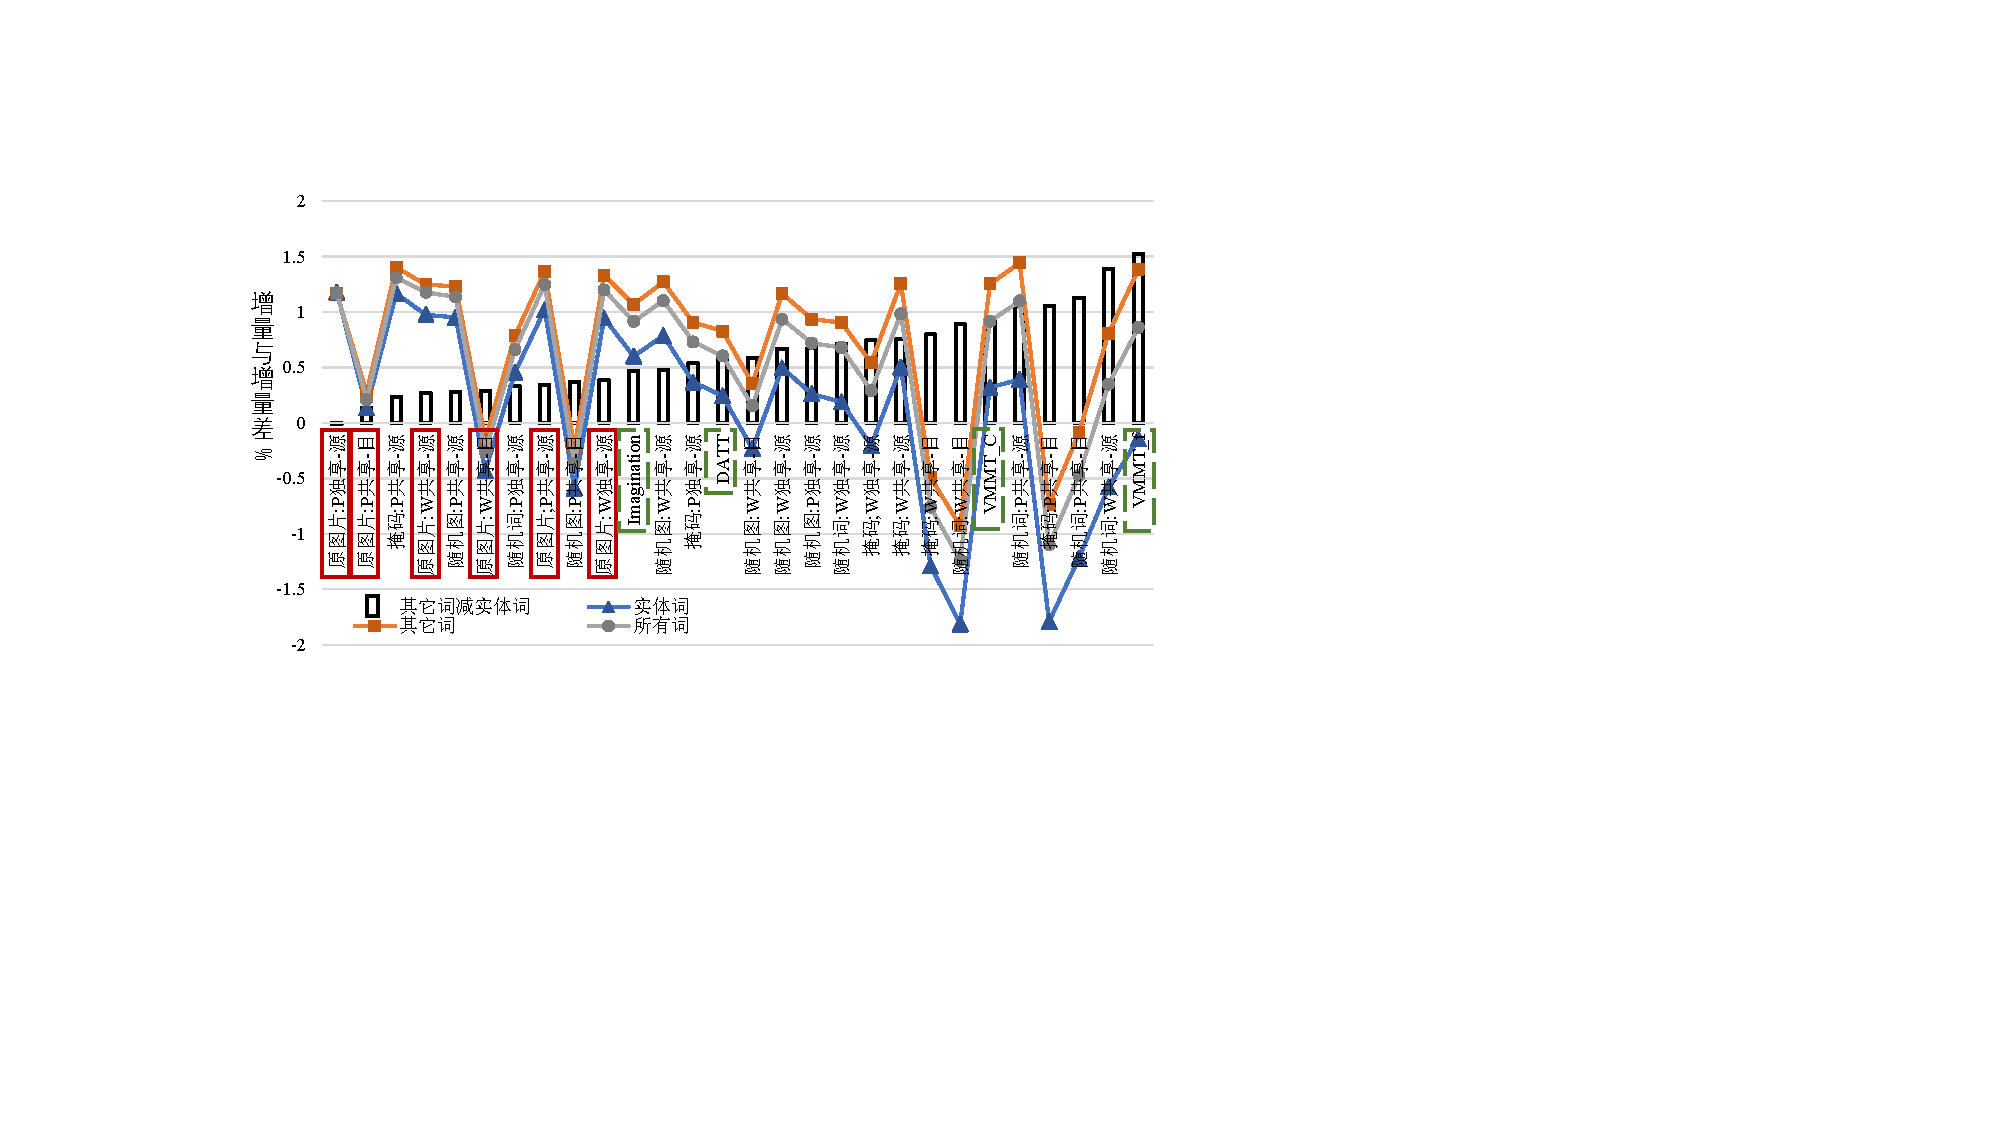
\includegraphics[scale=0.9]{Img/fig_3_analysis.pdf}
    \bicaption{实体词翻译准确率增量与增量差分析}{Accuracy increment and incremental difference analysis of entity words}
    \label{fig:3_analysis}
\end{figure}
本文选择在基于RNN的模型上进行比较。该结果需要每个方法提供模型的解码结果以及对应的纯文本基线模型的解码结果。比较的结果基于4种类型方法:6个本章的基于RNN的方法,12个\ref{sec:3_adversarial_ablation}小节中的对抗模型,6个\ref{sec:3_adversarial_ablation}小节中的掩码模型,以及4个\ref{tab:3_rnn_ende}表中的对比模型。实验结果中,本文同样测量了“所有词”的准确率,即不区分实体词或其它词的准确率。实验结果如图\ref{fig:3_analysis}所示,其中横轴代表不同的翻译系统,纵轴为增量值,蓝线代表实体词的增量值,红线代表其它词的增量值,灰线代表所有词的增量值,直方图代表其它词与实体词的增量值之差,本文称其为增量差(incremental difference)。

{\sffamily CTR-NMT:}图中实线框内的方法为本章所提CTR-NMT。图中一个值得注意的结果是,几乎所有的方法其它词的增量值都大于实体词的增量值。正如\ref{sec:3_setup_entity_extraction}小节所提到,多数实体词都是低频词,这导致模型更难学习这部分词的表示,所以当一个方法对神经翻译模型带来增益时,对所有词的提升是普遍现象,该提升也主要表现在其它词上,对实体词的提升主要依赖各类方法的特点。从图中直方图可以看到,本章所提方法的增量差普遍偏小,这说明该方法能够拉小了实体词与其它词之间增量值的差距,也就是为实体词带来的翻译准确率提升更多。

{\sffamily 对抗与消融方法:}从图中可以看出对抗评估和消融实验中所使用的模型普遍得到较高的实体词与其它词的增量值之差。没有证据表明降噪能力或多任务掩码方案能够帮助翻译中的实体词。这进一步证明了本章所提方法能够从视觉目标中提取有价值的视觉信息。

{\sffamily 对比模型方法:}DATT、$ \mathrm{VMMT_C} $、$ \mathrm{VMMT_F} $以及Imagination并没有明显地表现出降低实体词与其它词之间增量差的能力,以上整体的对比结果表明本章所提的显式跨模态信息融合方法能够有效地提升实体词的翻译准确率。

\subsection{样例分析}
\begin{figure}[!htbp]
    \centering
    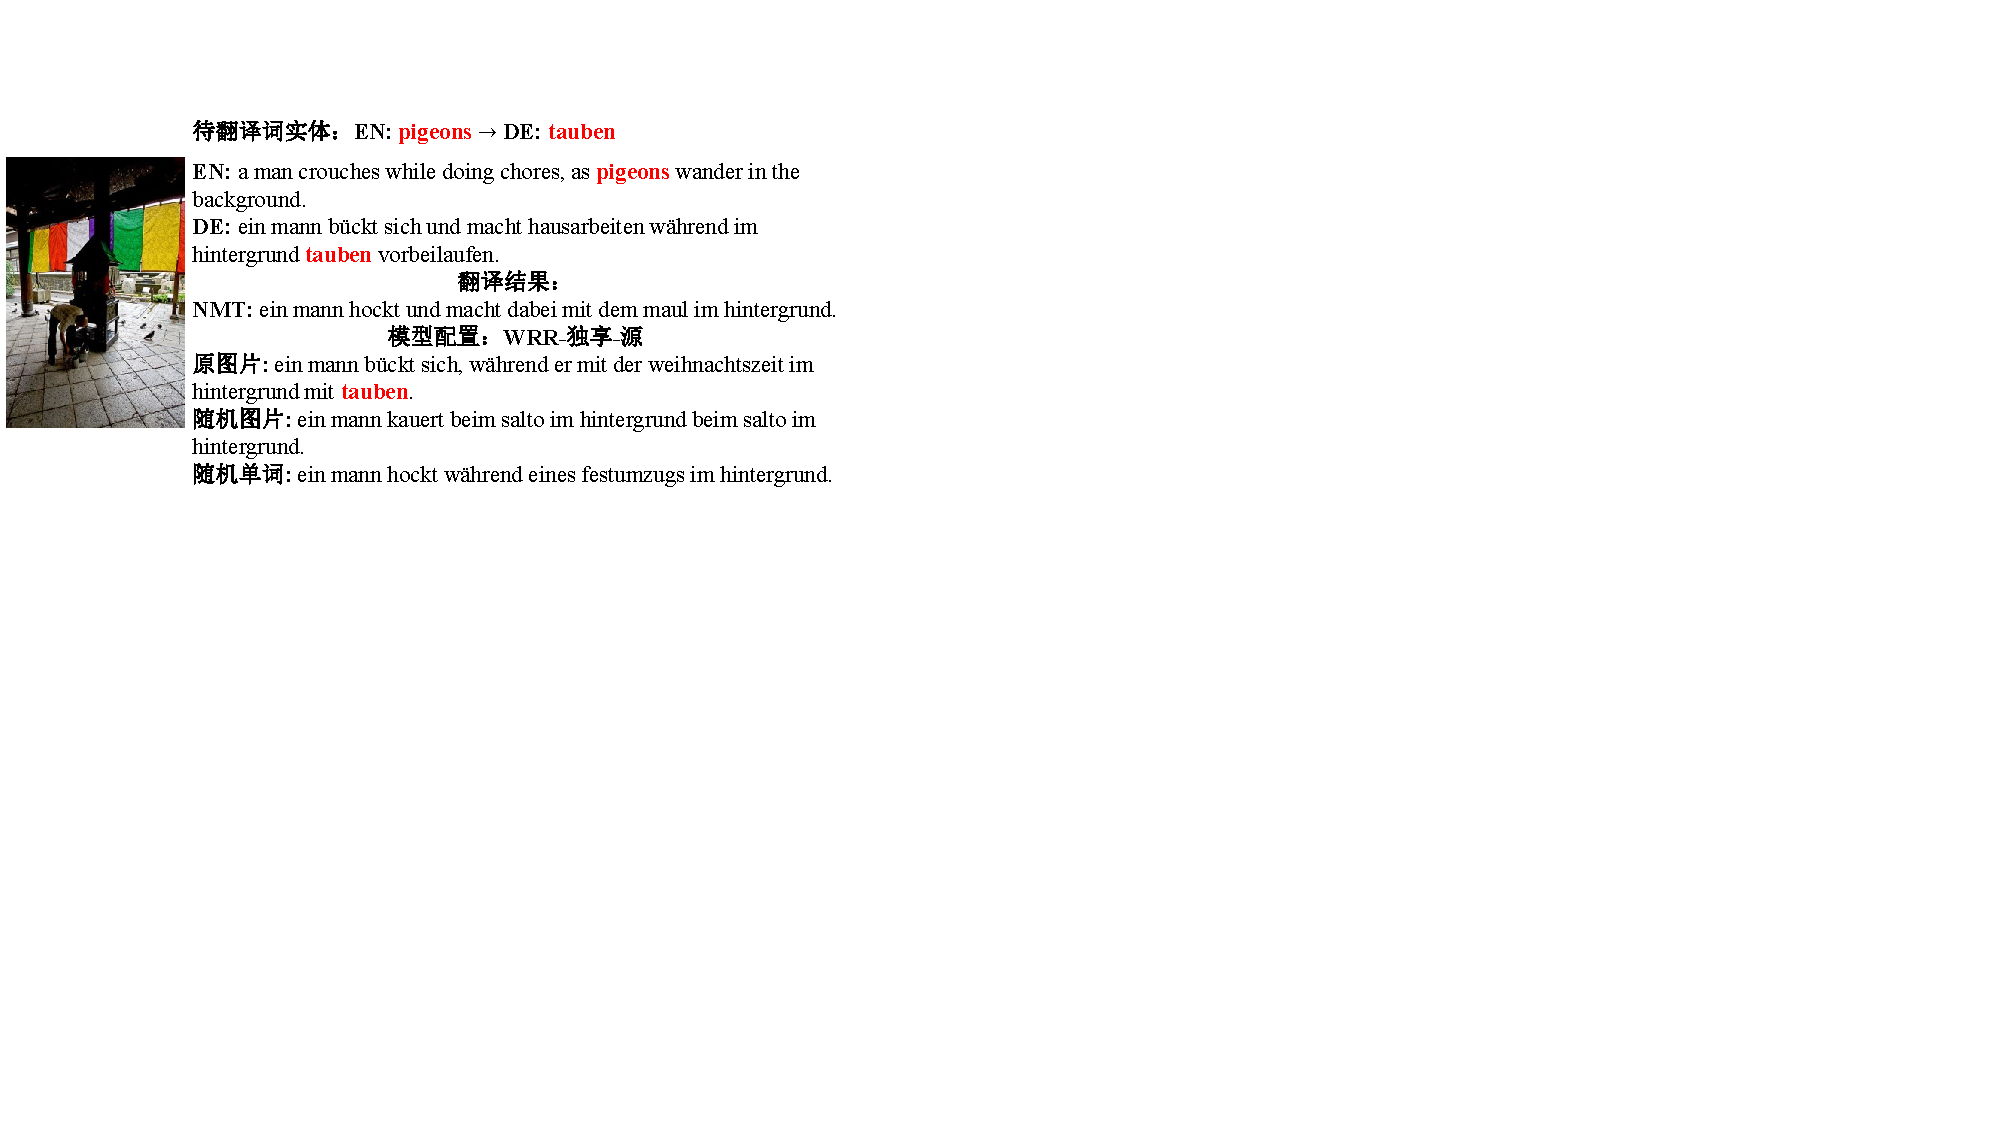
\includegraphics[scale=1.0]{Img/fig_3_case_1.pdf}
    \bicaption{实体词“pigeons”的翻译样例}{Translation example for the entity word "pigeons"}
    \label{fig:3_case_1}
\end{figure}
\begin{figure}[!htbp]
    \centering
    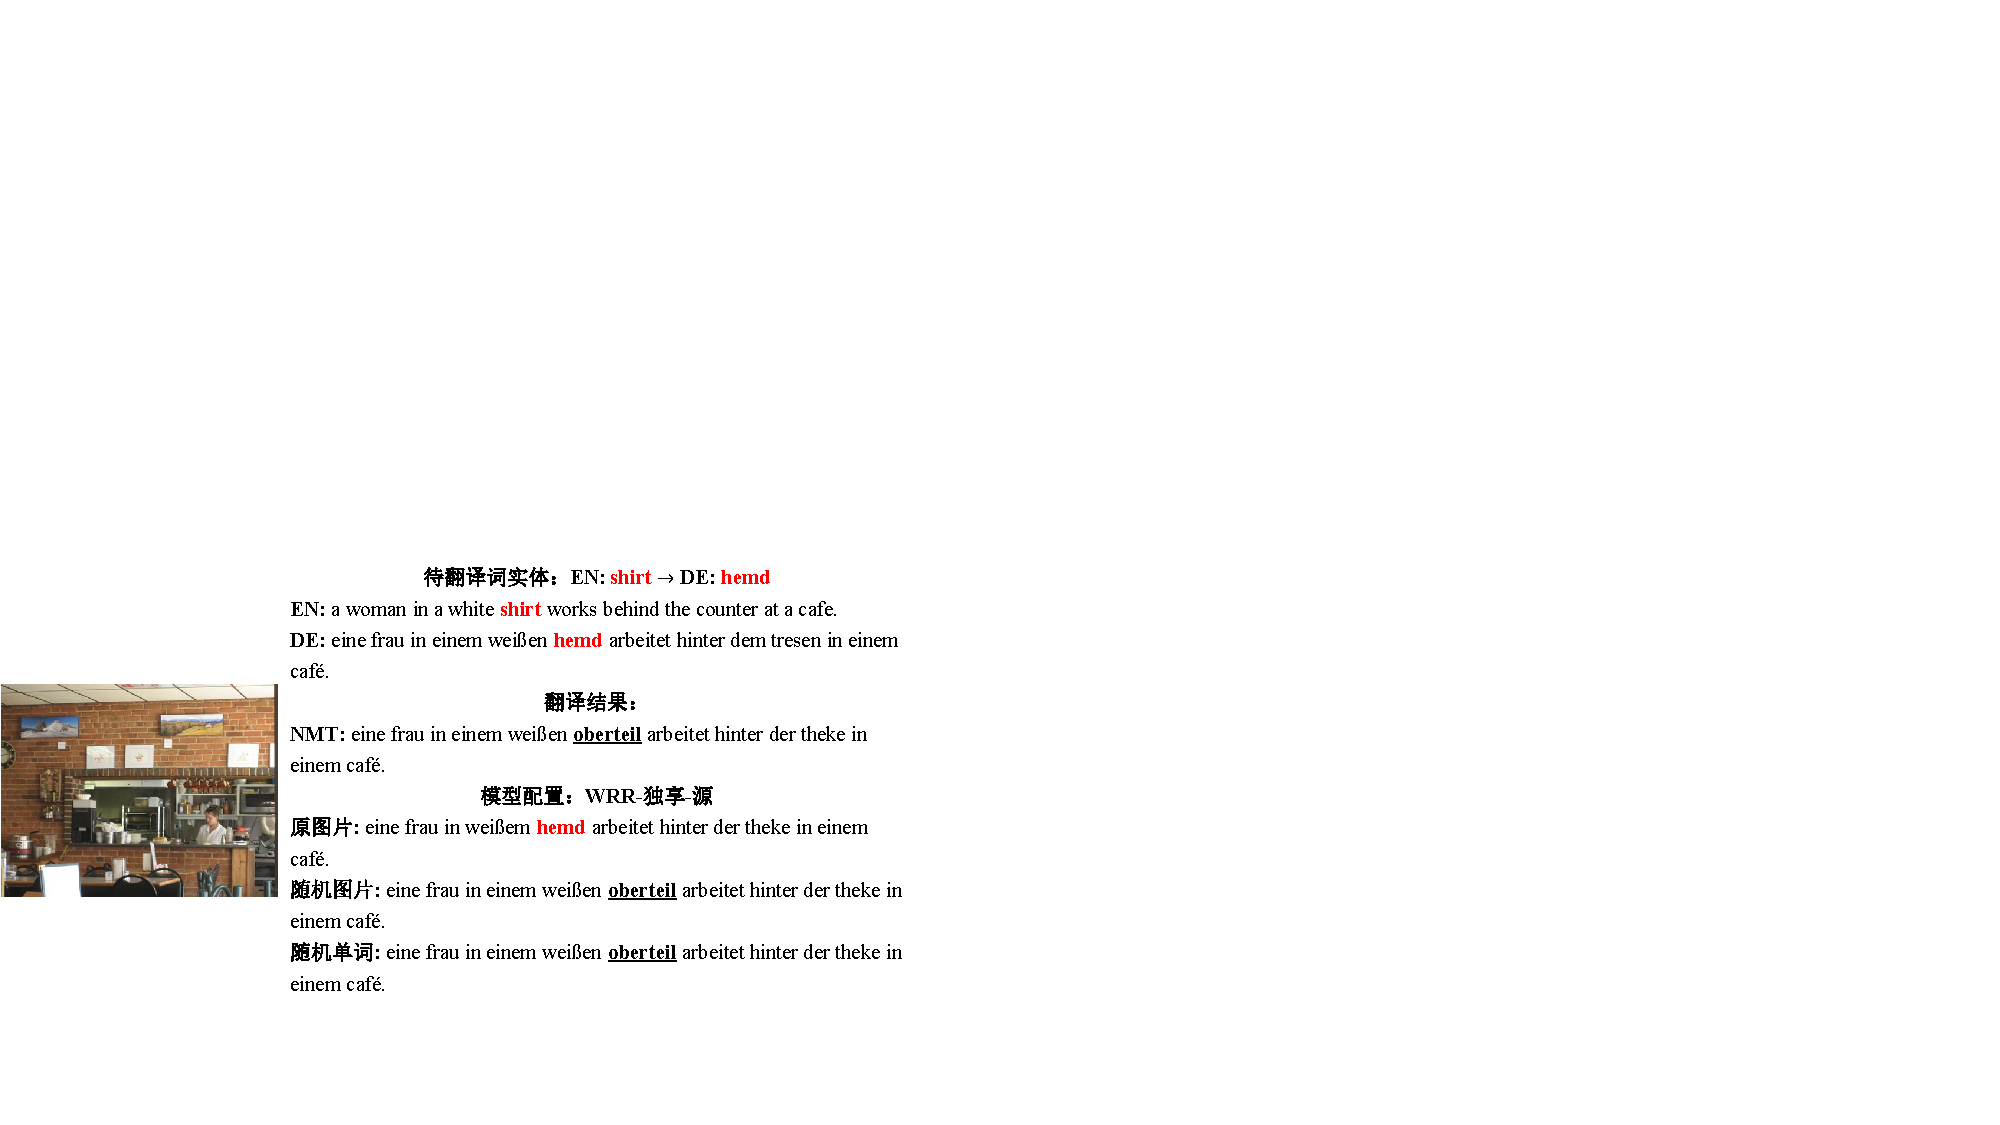
\includegraphics[scale=1.0]{Img/fig_3_case_2.pdf}
    \bicaption{实体词“shirt”的翻译样例}{Translation example for the entity word "shirt"}
    \label{fig:3_case_2}
\end{figure}
\begin{figure}[!htbp]
    \centering
    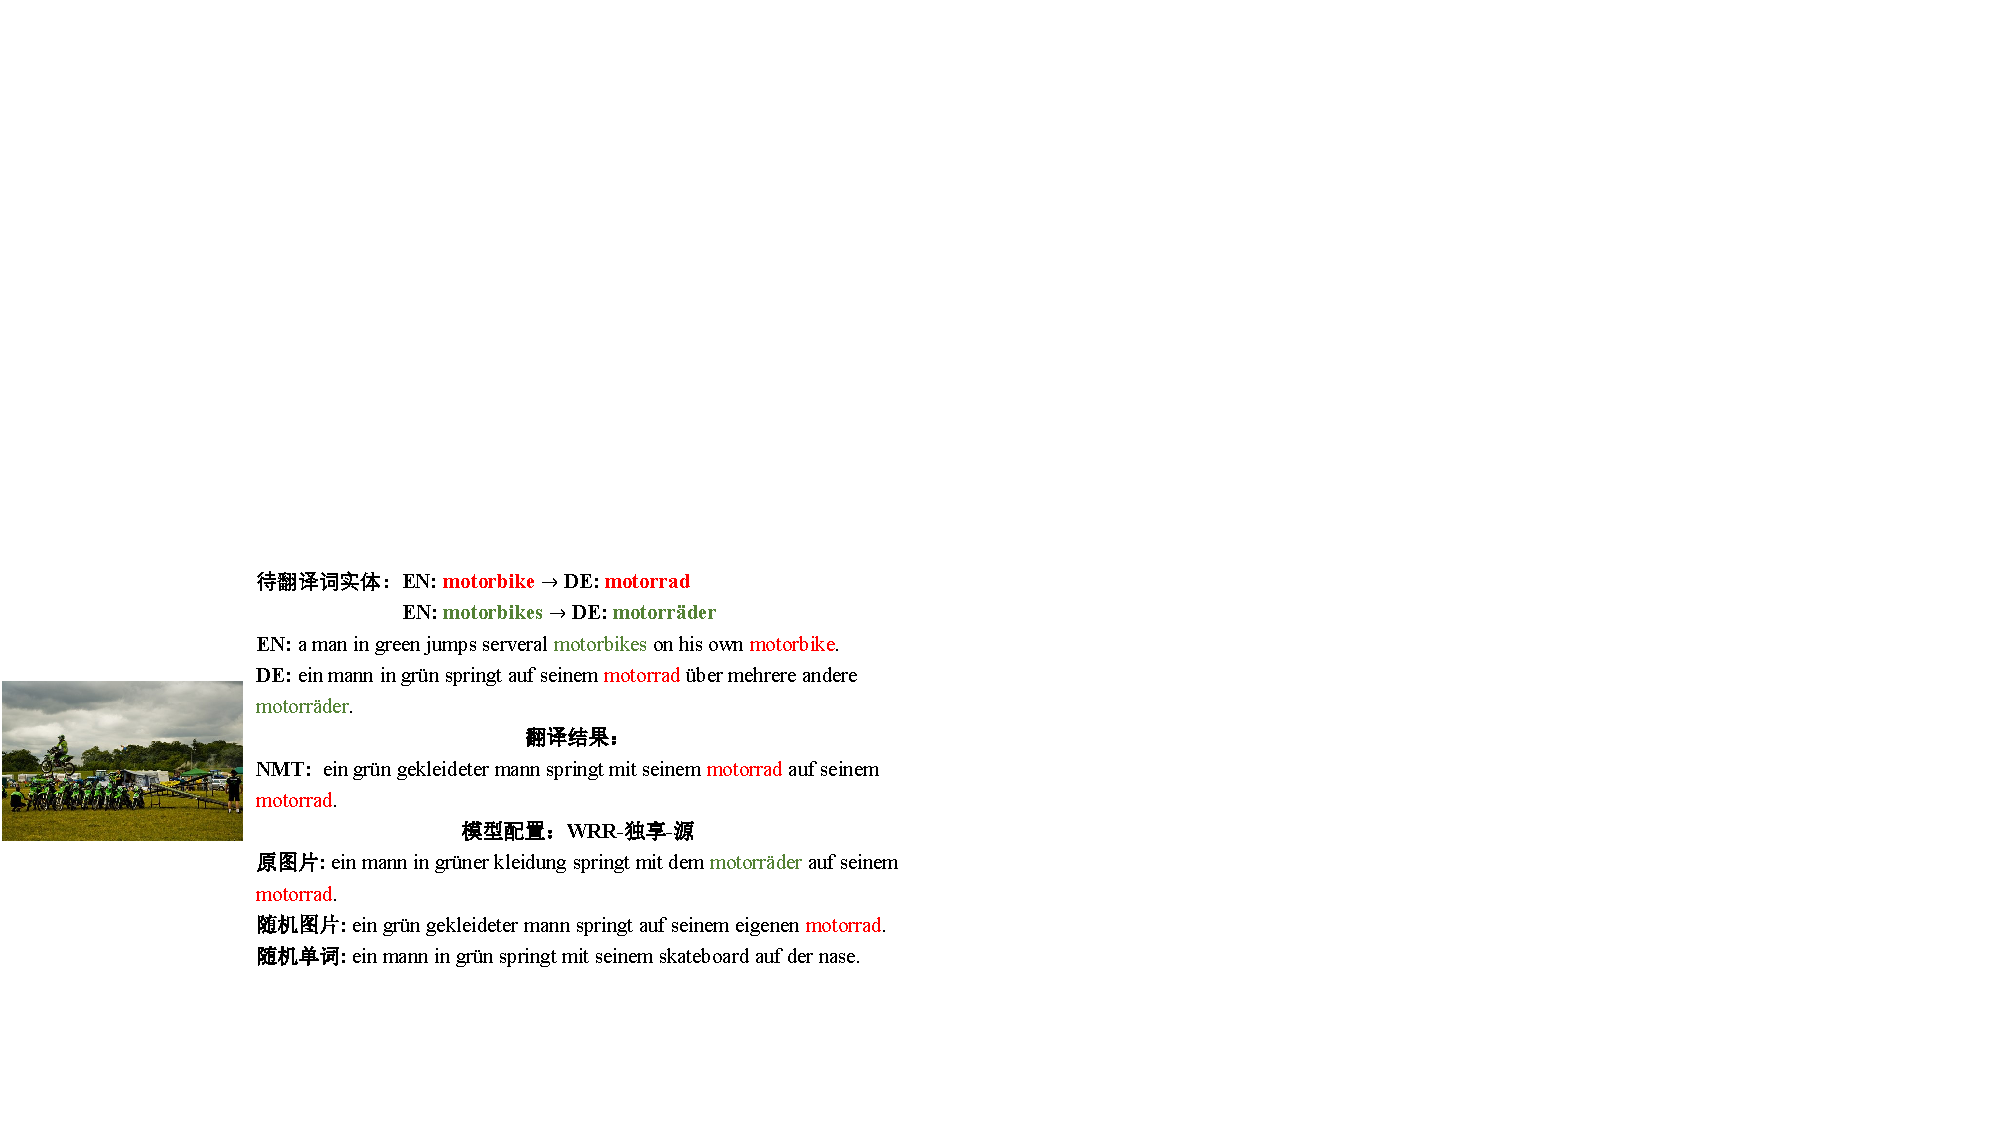
\includegraphics[scale=1.0]{Img/fig_3_case_3.pdf}
    \bicaption{实体词“motorbike”的翻译样例}{Translation example for the entity word "motorbike"}
    \label{fig:3_case_3}
\end{figure}
\begin{figure}[!htbp]
    \centering
    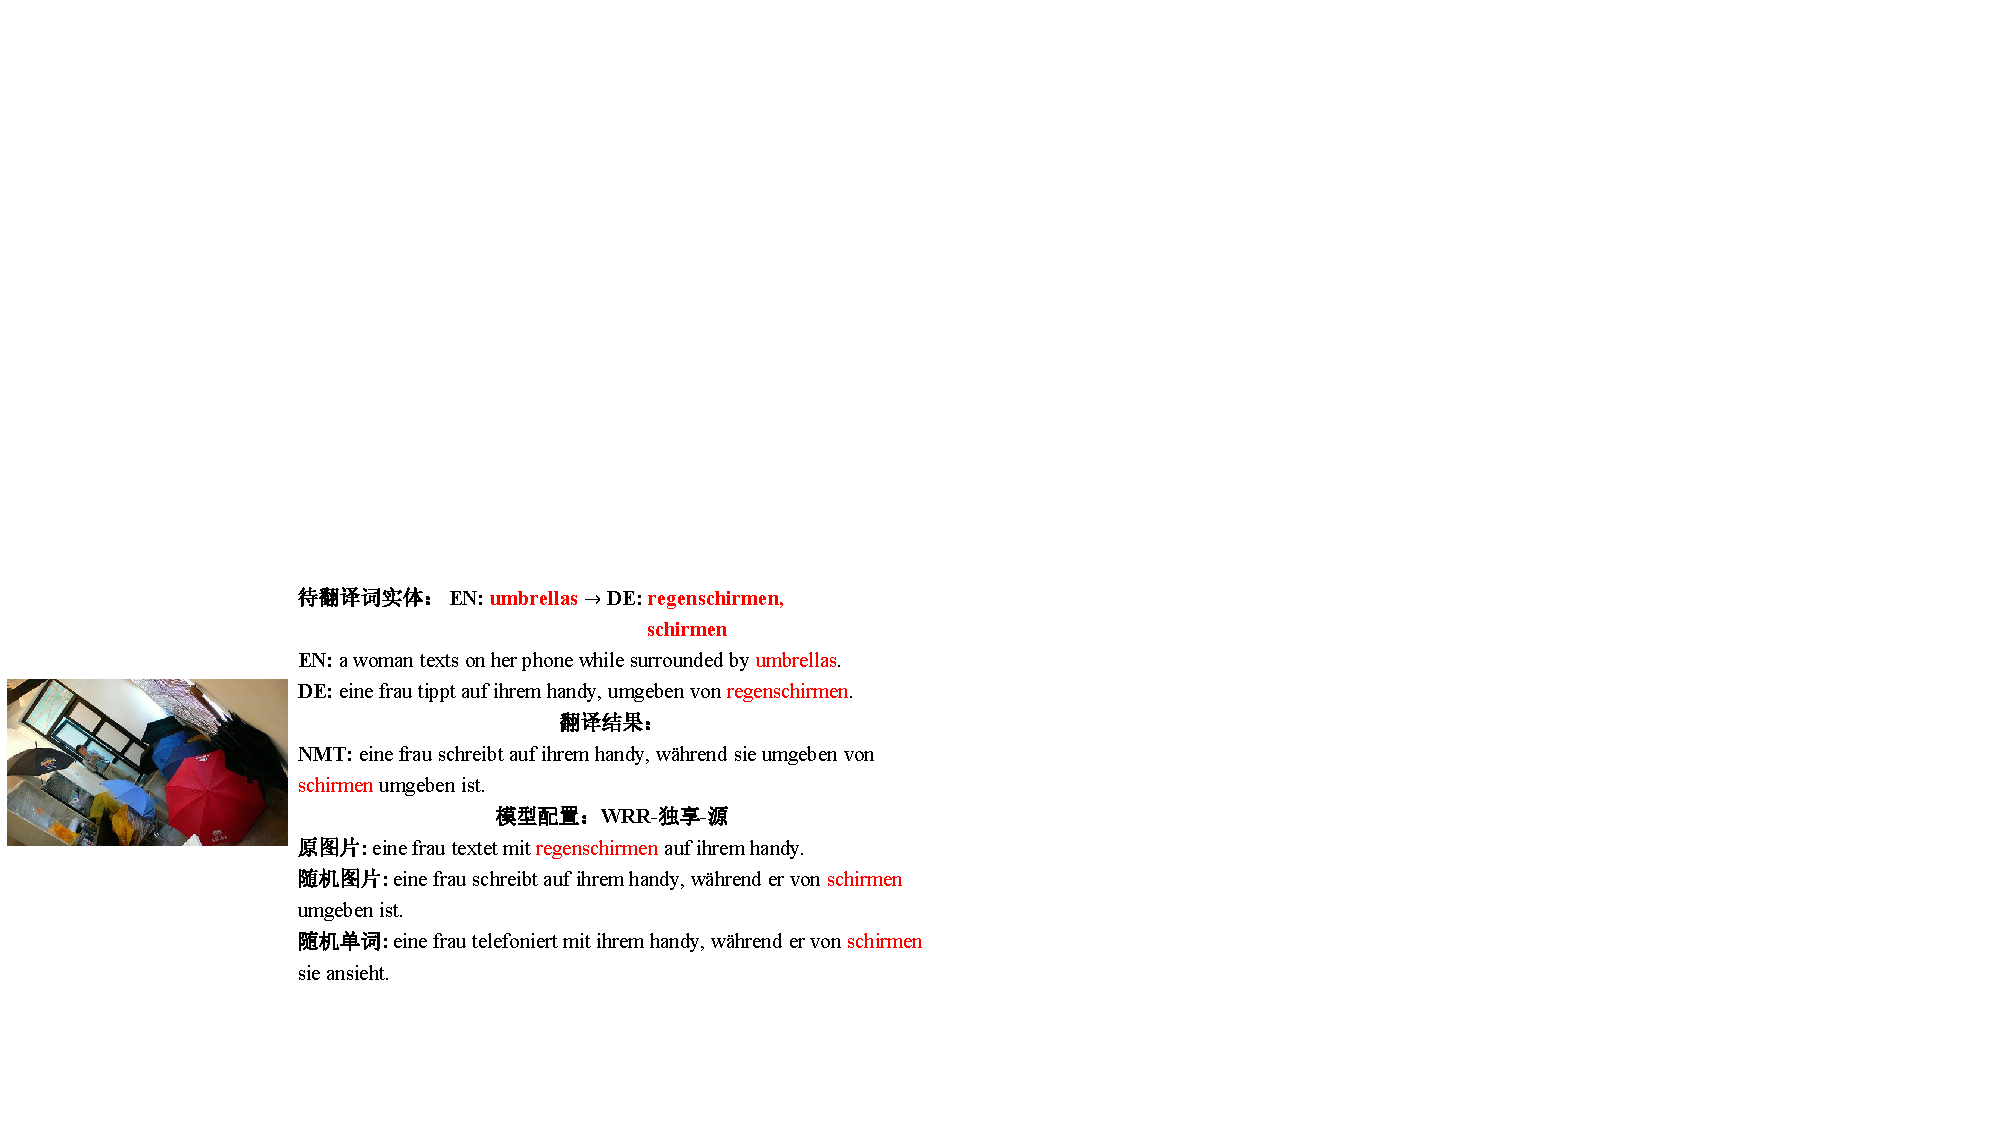
\includegraphics[scale=1.0]{Img/fig_3_case_4.pdf}
    \bicaption{实体词“umbrellas”的翻译样例}{Translation example for the entity word "umbrellas"}
    \label{fig:3_case_4}
\end{figure}
为了展示本章所提方法对句子翻译和实体词翻译带来的影响,本文在图\ref{fig:3_case_1}至\ref{fig:3_case_4}中展示了4个翻译案例。其中包含着实体词“pigeon”、“shirt”、“motorbike”和“umbrellas”的翻译。通过观察可以得到以下结论:输入正确的图片信息时,模型的性能表现相对较好;当实体词有多种释义时,其它模型的翻译结果在多个释义上容易表现出不稳定的结果,本章所提方法的表现更好。

\section{本章小结}
为了探究显式跨模态信息融合方法的可行性,本章提出了一种以明确的方式将文本中的短语或名词替换文图片中相对应的视觉目标。然后将该方法应用于文本句子的重构任务,再通过参数共享的方式,将重构模型优化后的模型参数与翻译模型共享,从而增强了神经机器翻译系统的翻译性能。
该方法在融合图片信息的翻译任务常用的Multi30K英德翻译对上进行了实验,在测试阶段不需要输入图片的情况下,在基于循环神经网络的模型中取得了最佳的翻译效果,在基于Transformer的模型上与其它模型仍然是可比的。
在消融与对抗训练的实验中,输入原图片的模型相比于输入随机噪声或不输入图片的掩码方案翻译性能最佳。说明文本重构模型通过利用图片信息优化了模型的参数,使翻译模型得到了增强。
在进一步的实验分析中发现,本章所提方法主要提升了实体词的翻译准确率,从而在整体上提升了译文的质量。该研究成果发表于2021年自然语言处理实证方法会议(EMNLP 2021)。

%为了探究显式跨模态信息融合的可行性,本章提出了一种以明确的方式将图片中的视觉目标信息与文本中对应的短语实体或词实体相融合的方法。并将该方法应用于文本的重构任务,最后通过多任务参数共享的方式,优化了翻译模型中对实体词的翻译能力,从而带来了进一步翻译质量的提升。实验结果表明,所提方法在测试阶段不需输入图片信息的条件下依旧与其它需要输入图片的方法是可比的,并且对词实体的翻译具有显著的提升作用。该研究成果发表于Findings of the Association for Computational Linguistics: EMNLP 2021。